%************************************************
% BACKGROUND
%************************************************

\chapter{Background} \label{chap: background}

\paragraph{} \textit{This chapter explains the theory behind the methods and techniques used in this project: it begins by describing the EEG data and presenting a formal definition of the problem; later, it presents logistic regression and the related evaluation metrics, followed by the description of activation functions, optimizers and regularizers used in the project; subsequently, it describes the classic machine learning models and deep learning models used and, finally, it presents the the functional connectivity, the graph representation and the graph-based deep learning models.}

\section{Epileptic seizures and EEG} \label{sec: epileptic_seizures_and_eeg}
\paragraph{} An epileptic seizure is a disruption of the electrical signals in our brain \cite{EpilepsySociety:aboutepilepsy}. The brain controls the way we function millions of neurons, which pass messages to each other by electrical signals. If these signals are disrupted, our body and feelings are hugely influenced by this change.

Since epileptic seizures arise inside the brain, the most common tests that specialist use in order to diagnose epilepsy are the electroencephalogram (EEG) and MRI (brain scans). Neither of these tests is able to confirm for certain if the patient has epilepsy or not, but they can help the specialist to decide whether to consider epilepsy as possible diagnosis. We are going to focus on the EEG, since the project is based on a dataset of iEEGs.

EEG gives an overview of the activity of the brain cells, that is the traffic of nerve impulses that neurons send each other to communicate, also called \textit{brain waves}. The messages between neurons consist of changes in the electrical charge of the cells: when a neuron sends a message, it "gives off" electricity. In the EEG test, the brain waves are picked up by electrodes, which are small sensors placed on different areas of the patient's head. When the electrodes are placed directly on the surface of the brain, we talk about \textit{intracranial electroencephalogram} (iEEG). The electrodes are able to record the electrical activity from small areas of the brain, therefore each electrode outputs an electrical signal that varies over time. The EEG is the combination of all the electrodes signals in one single "chart", where we can see a signal for each electrode (y-axis) vary over time (x-axis). Figure \ref{fig:eeg_example} shows an example of an EEG, which in this case presents some epileptic spikes.

\begin{figure}[htbp]
    \centering
    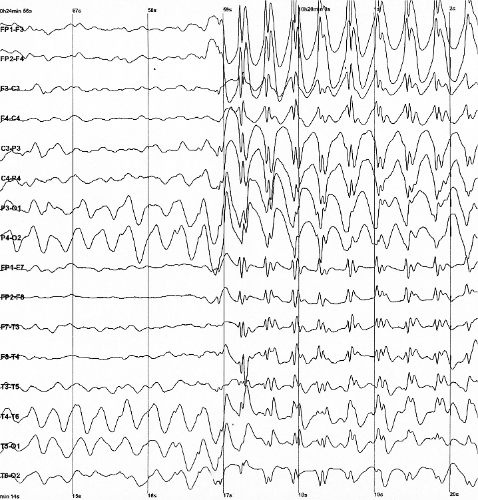
\includegraphics[width=0.6\textwidth]{eeg_example}
    \caption{Example of epileptic spikes monitored with EEG (from \textit{Wikipedia, the free encyclopedia})}
    \label{fig:eeg_example}
\end{figure}

The number of electrodes used can range from a few dozen to hundreds. They are positioned on specific sections of the patient's head, therefore different electrodes monitor the activity of different areas of the brain. In this way, by looking at the EEG and knowing the position of each electrode, the specialist can understand which areas of the patient's brain are involved in the seizure. The electrodes are identified based on whether they are placed on the left or right side of the head and also based on the lobe they are recording from (frontal lobes, temporal lobes, parietal lobes or occipital lobes). The EEG monitoring captures several types of brain waves, which differ in the frequency (waves per second). Specific ranges of frequencies are determined by particular moments of the day, situations and states of mind.

The EEG is a very helpful tool for epilepsy diagnosis, but it can't show for certain the presence of epileptic seizures. In fact, despite the existence of typical signal patterns associated with epilepsy, usually epileptic seizures look very different on the EEG depending on the patient: some seizures are recognizable thanks to the presence of typical spikes in the electrical signals; other seizures happen without showing any visible change in the EEG. Therefore, we have reason to think that for some patients the seizure is "hidden" in the relations between signals behaviour, more than in the behaviour of each signal itself. Even when the change in the EEG pattern is clear, it could involve only a subset of electrodes (partial seizures) or all the electrodes (generalized seizures), and it is difficult to determine if the disruption of the signal is actually caused by epilepsy or if it simply represents an 'abnormal' EEG, which could happen without the presence of seizures.

\section{Problem definition} \label{sec: problem_definition}
\paragraph{} The focus of this thesis is on the seizure prediction problem, but we are going to analyze also the seizure detection task in order to have a clearer and more complete idea of the machine learning models potentialities on epileptic seizures data.

The seizure prediction/detection problem can be treated as a classification problem, whose aim is to predict a class associated with each sample. In the case of an EEG, if we consider discrete instants of time, we can represent the EEG information as a matrix $N \times F$, where the rows represent the $N$ electrodes and the columns represent the features associated with the $F$ time instants. So, for each of the $N$ electrodes, we have a sequence of $F$ values representing the amplitude over time. The task can be treated as a classification problem by associating each time instant with a label or target, which represents the class of membership between \textit{seizure} and \textit{non-seizure}. This means that each time instant is classified based on the presence or absence of an ongoing epileptic seizure in that instant. If we indicate with $x_t$ the set of signals features related to a single time instant, we can say that each time instant $t$ with features $x_t$ has an associated target $y_t$, which is equal to $1$ if there is an ongoing seizure and to $0$ otherwise. Thus considered, the seizure prediction/detection problem becomes the task of predicting the class target $y_t$ related to the time instant features $x_t$.

\begin{figure}[htbp]
    \centering
    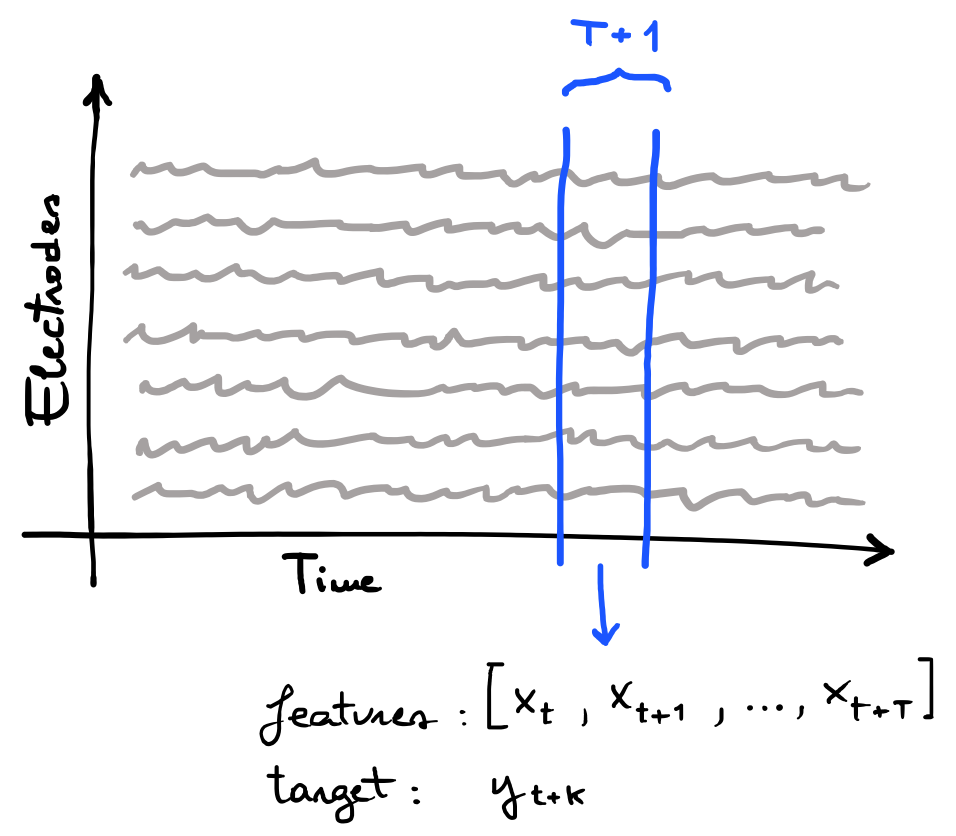
\includegraphics[width=0.6\textwidth]{problem_def}
    \caption{Problem definition}
    \label{fig:problem_def}
\end{figure}

Let's consider a time portion of $T+1$ discrete instants in an EEG: the portion will be characterized by a sequence of features $[x_t, x_{t+1}, x_{t+2}, ... , x_{t+T}]$, one for each time instant $t$, representing the signals amplitude (measured in volts) in that instant. Let's imagine that the time portion is used to predict a single target $y_{t+k}$, which indicates whether the instant $t+k$ is part of an ongoing epileptic seizure or not. The described situation is illustrated in Figure \ref{fig:problem_def}. Considering this scenario, we can individuate three cases of study of the problem, depending on the value of the variables $T$ and $k$:
\begin{itemize}
    \item $T=0,\quad k=0$: in this case, the length of the time portion is equal to $1$ and the target corresponds to label of the same time instant of the sample. So at each sample $x_t$ is associated the target $y_t$ (as in the case described above).\\
    \textsc{Example:} \quad$T=0, k=0\quad \Rightarrow{}\quad [x_3] \rightarrow{} y_3$
    \item $T>0,\quad k=T$: in this case, the length of the time portion is greater that $1$, so it consists of a sequence of samples, and the target is the label associated to the last sample of the sequence. So at each sequence $[x_t, x_{t+1}, ... , x_{t+T}]$ is associated the target $y_{t+T}$.\\
    \textsc{Example:} \quad$T=5, k=5\quad \Rightarrow{}\quad [x_0, x_1, ..., x_5] \rightarrow{} y_5$
    \item $k>T$: in this case, we have a sequence of samples whose target is associated to a sample that doesn't belong the sequence, but is forwards in time ($t>T+1$). This means that at each sequence $[x_t, x_{t+1}, ... , x_{t+T}]$ is associated the target $y_{t+k}$, where $(t+k) > (t+T)$.\\
    \textsc{Example:} \quad$T=5, k=8\quad \Rightarrow{}\quad [x_0, x_1, ..., x_5] \rightarrow{} y_8$
\end{itemize}
The first two cases are examples of a detection problem, since the target $y_{t+k}$ to predict is associated to an instant that is still inside the time window we look at to predict it ($k \leq T$). The third case, on the other hand, is a prediction problem, since the target $y_{t+k}$ to predict is associated to an instant that is outside the time window we look at to predict it and it is forwards in time with respect to the time window ($k > T$). The difficulty of the prediction task is that we cannot look at the features $x_t$ in order to predict the target $y_t$, but we have to rely on information from previous timestamps (for this reason, we consider $T>0$, since it would be almost impossible to predict the target based on a single sample backwards in time).

\section{Logistic Regression} \label{sec: logistic_regression}

\paragraph{} In this project, the binary classification problem related to epileptic seizure detection/prediction is approached using logistic regression. The logistic regression algorithm is used to estimate the probability that an instance belongs to a particular class \cite{OReilly:handsonML}. If the estimated probability is greater than a fixed threshold, which is commonly set to $0.5$, then the model assigns the instance to the positive class (in our case, \textit{seizure} class), otherwise it assigns the instance to the negative class (in our case, \textit{non-seizure}). In this way, logistic regression can be used as a binary classifier.

Let's look at a very simple logistic regression model as an example: it computes the weighted sum of the input features $\mathbf{x}$ multiplied to the model parameter $\theta$ and it outputs the logistic of the result:
\begin{align}
    \hat{p} = h_{\theta}(\mathbf{X}) = \sigma\left(\theta^T \mathbf{x}\right)
\end{align}
The logistic $\sigma$ is a sigmoid function that generates a number between $0$ and $1$, representing the probability $\hat{p}$ that an instance $\mathbf{x}$ belongs to the positive class. The sigmoid function is illustrated in Figure \ref{fig:sigmoid} and it is mathematically defined as:
\begin{align}
    \sigma(t) = \frac{1}{1 + \exp{(-t)}}
\end{align}

\begin{figure}[htbp]
    \centering
    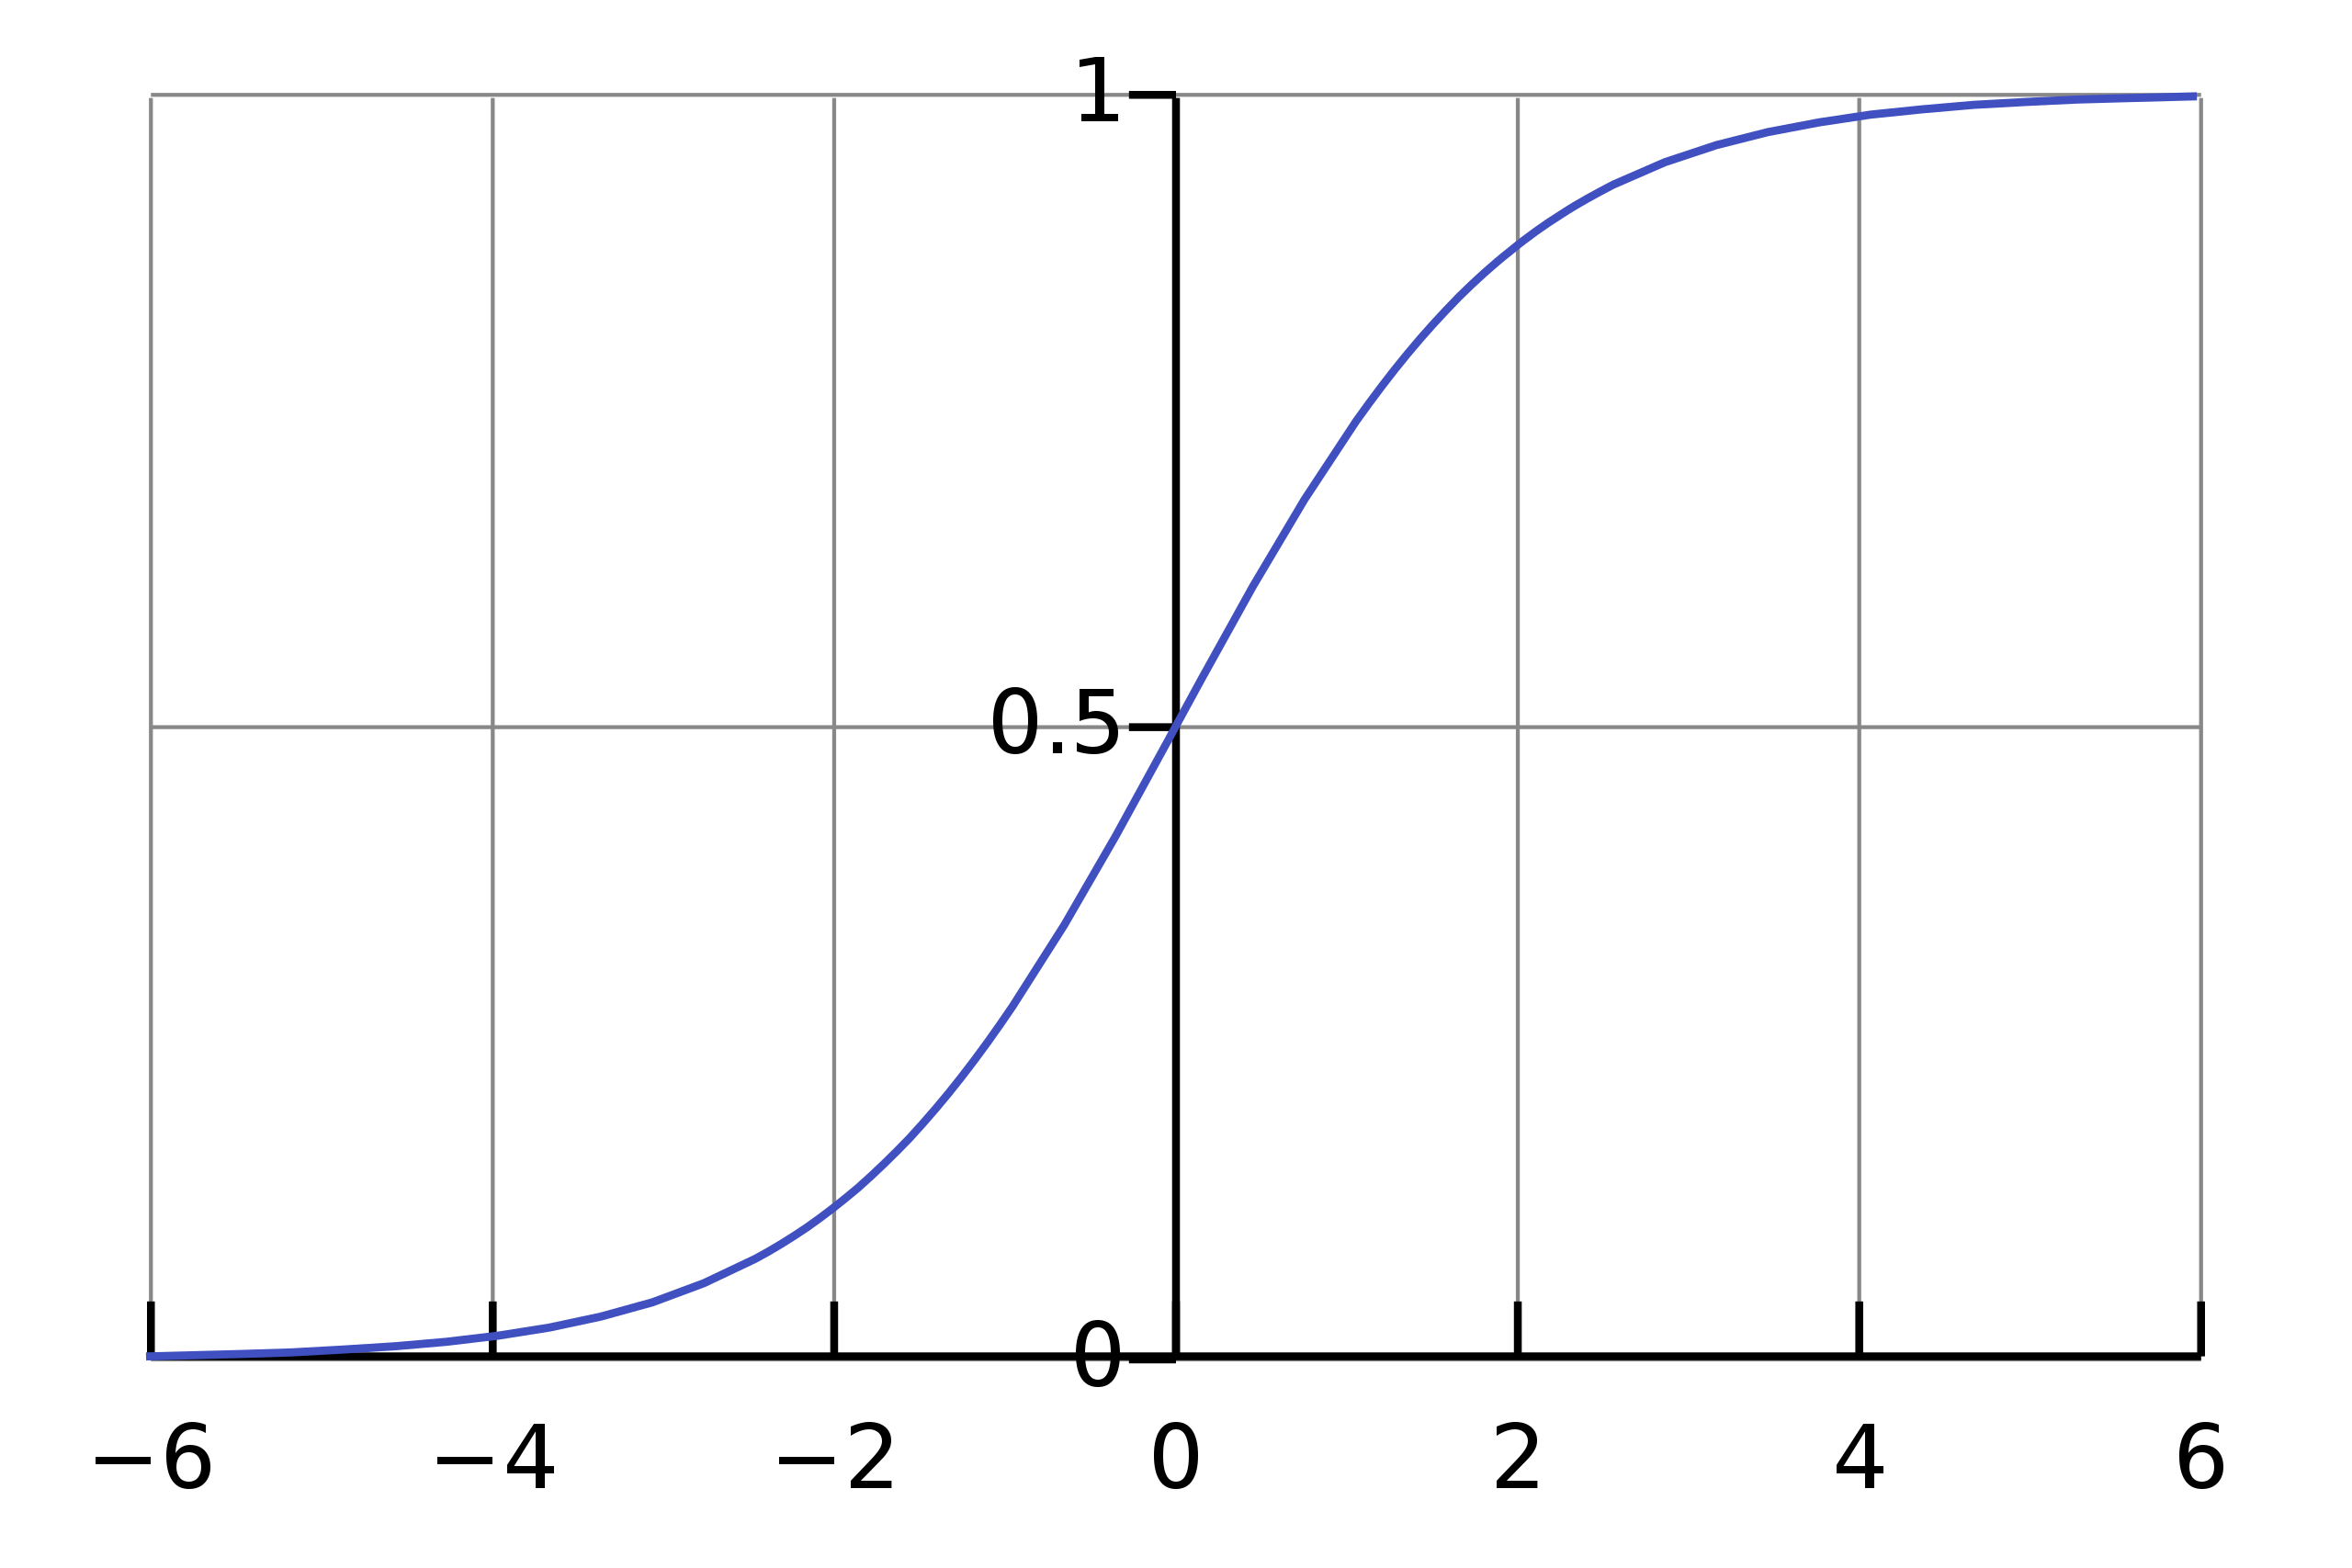
\includegraphics[width=0.6\textwidth]{sigmoid}
    \caption{Sigmoid function (from \textit{Wikipedia, the free encyclopedia})}
    \label{fig:sigmoid}
\end{figure}

The predictions $\hat{y}$ for the binary classifier can be easily obtained by applying the following equation to the probability $\hat{p}$:
\begin{align}
    \hat{y} = \left\{\begin{array}{l}{0 \text { if } \hat{p}<0.5} \\ {1 \text { if } \hat{p} \geq 0.5}\end{array}\right.
\end{align}

The model parameter $\theta$ is trained in order to estimate high probabilities for positive instances and low probabilities for negative ones. In order to train it, we need a cost function that directs the model on the right track. For logistic regression algorithms, the most suitable cost function is the \textit{log loss}, since it captures exactly the aim of the classifier:
\begin{align}
    c(\theta) = \left\{\begin{array}{ll}{-\log (\hat{p})} & {\text { if } y=1} \\ {-\log (1-\hat{p})} & {\text { if } y=0}\end{array}\right.
\end{align}
$-\log (\hat{p})$ becomes higher and higher and tends toward infinity the more $\hat{p}$ get close to $0$, while it gets near to $0$ when $\hat{p}$ approaches $1$. $-\log (1-\hat{p})$ behaves in the opposite way, so it makes sense to use the first one for the positive class and the second one for the negative class. The cost function is applied to multiple training instances by computing the average cost over all the $n$ instances:
\begin{align}
    \textit{error } = -\frac{1}{n} \sum^{n}_{i=1}\left[y_i \log(\hat{p}_i) +
    (1 - y_i) \log(1 - \hat{p}_i)\right]
\end{align}
The log loss cost function is then used by an optimizer, for instance Gradient Descent or Root Mean Square Propagation algorithms, in order to update the model parameters accordingly. Usually, like in this project, the optimizer works on mini-batches, so the model parameters are updated after each mini-batch.

The project models make use of the same process, but instead of using such a simple model consisting of only one parameter, we used a set of more complex machine learning models and applied logistic regression to each of them to build several binary classifiers.

\section{Metrics} \label{sec: metrics}
\paragraph{} In order to evaluate the models, four metrics have been chosen, which are commonly used for binary classifiers: loss, accuracy, ROC-AUC and recall. The first two metrics are the most standard performance measures for all the machine learning models.

\paragraph{Loss} The loss is nothing but the error computed by the cost function in use, which in our case is the log loss.

\todo[inline]{Add description of brier\_score\_loss (used for classic ml models)}

\paragraph{Accuracy} The accuracy is simply the ratio of correct prediction, which in a binary classifier is represented by the number of true prediction (true positive and true negative) over the total number of predictions:
\begin{align}
    \textit{acc } = \frac{(TP + TN)}{(TP + TN + FP + FN)}
\end{align}
where \textit{TP} = true positive, \textit{TN} = true negative, \textit{FP} = false positive, \textit{FN} = false negative.

\paragraph{Recall} The recall, also called sensitivity or true positive rate, is the number of positive instances correctly classified over the total number of positive instances:
\begin{align}
    \textit{recall } = \frac{(TP)}{(TP + FN)}
\end{align}

\paragraph{ROC-AUC} The ROC curve (receiver operating characteristic curve) is a plot of the true positive rate (recall) against the false positive rate (shown in Figure \ref{fig:roc_auc}):
\begin{align}
    \textit{TPR } = \frac{(TP)}{(TP + FN)} \qquad\qquad \textit{FPR } = \frac{(FP)}{(FP + TN)}
\end{align}
The false positive rate is the number of negative instances incorrectly classified as positive over the total number of negative instances.
\begin{figure}[htbp]
    \centering
    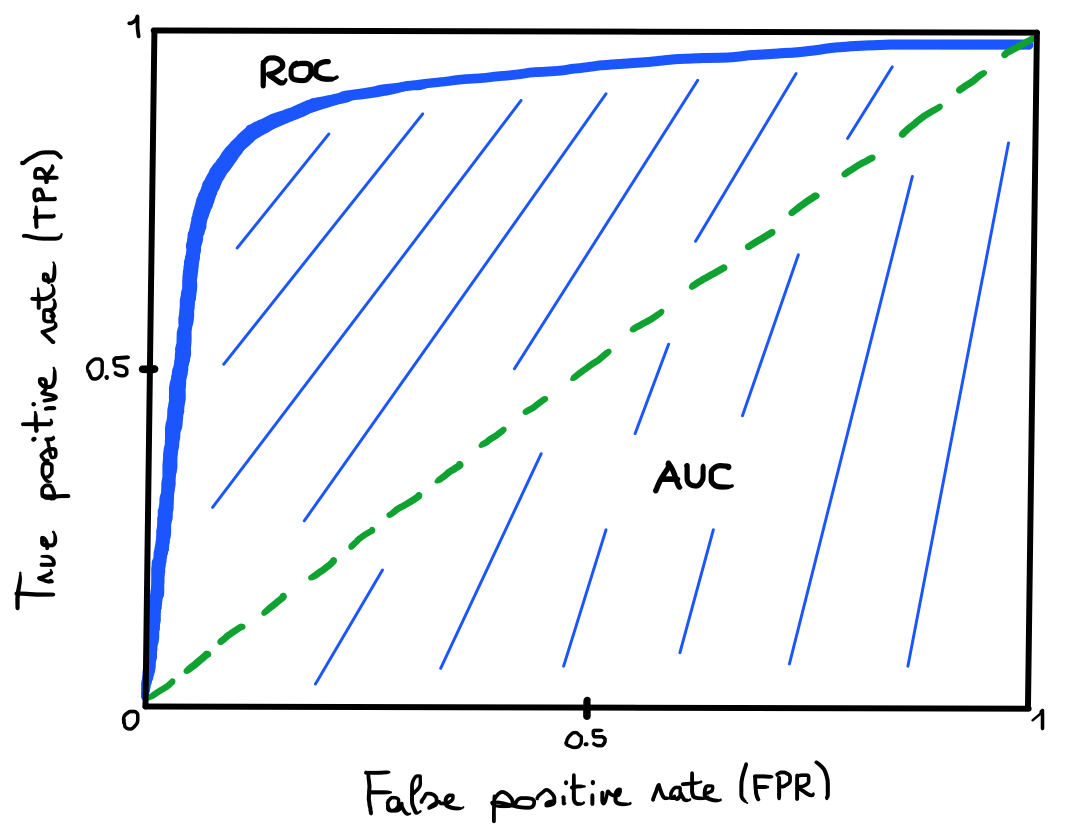
\includegraphics[width=0.6\textwidth]{roc_auc}
    \caption{ROC curve and respective AUC}
    \label{fig:roc_auc}
\end{figure}

The ROC curve represents a plot of TPR and FPR at different classification thresholds: if we lower the threshold, the classifier predicts more items as positive, so both TPR and FPR increase. In order to find the best classification threshold, we need to find a tradeoff between TPR and FPR, trying to obtain a higher TPR as possible and a lower FPR as possible (looking at the curve, we need to find the point that is closest to the upper left corner). For this purpose we can rely on the \textit{area under the ROC curve} (AUC), which provides a performance measure for different classification thresholds. The ROC-AUC ranges
from 0 to 1 and its value represents the quality of the classifier predictions. A perfect classifier has AUC = 1, while a completely random classifier has AUC = 0.5.

\section{Activation, optimization and regularization} \label{sec: activation_optimization_regularization}
\paragraph{} This section describes topics that are related only to the deep learning models.

\subsection{Activation functions}
An activation function is a non-linear mapping between the input and the output. Activation functions are essential in neural networks layers, since they introduce the non-linearity properties to the model: without activation functions, the neural network would be a simple linear transformation and it wouldn't be able to learn from complex data.

Some activation functions are more suited to hidden layers, while others are perfect to compute the final output of the model. In this project, we used the sigmoid function as activation function for the last layer of our models in order to classify data, as previously explained in Section \ref{sec: logistic_regression}. For the hidden layers, we used both ReLU and Tanh activation functions.

\paragraph{ReLU} ReLU (Rectified Linear Unit) is a very popular and extremely fast and effective activation function for hidden layers. Its principle is very simple: it keeps only positive values, while setting to 0 all the negative ones.
\begin{align}
    \text{R}(x) = max(0, x)
\end{align}
The ReLU function is illustrated in Figure \ref{fig:relu}.

\paragraph{Tanh} Tanh (Hyperbolic Tangent) is similar to sigmoid, but it ranges from $-1$ to $1$. It maps negative input as strongly negative, positive ones as strongly positive and zero inputs near zero. Its formula is:
\begin{align}
    \tanh{(x)} = \frac{e^{2x} - 1}{e^{2x} + 1}
\end{align}
The Tanh function is illustrated in Figure \ref{fig:tanh}.
\begin{figure}[htbp]
    \centering
    \begin{subfigure}[t]{0.5\textwidth}
		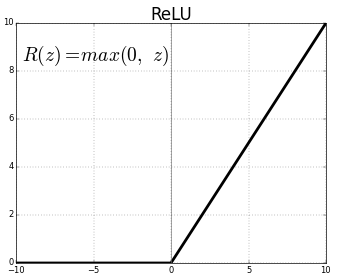
\includegraphics[width=0.9\textwidth]{relu}
        \caption{ReLU activation function (from \textit{Medium})}
        \label{fig:relu}
	\end{subfigure}%
	~
	\begin{subfigure}[t]{0.5\textwidth}
		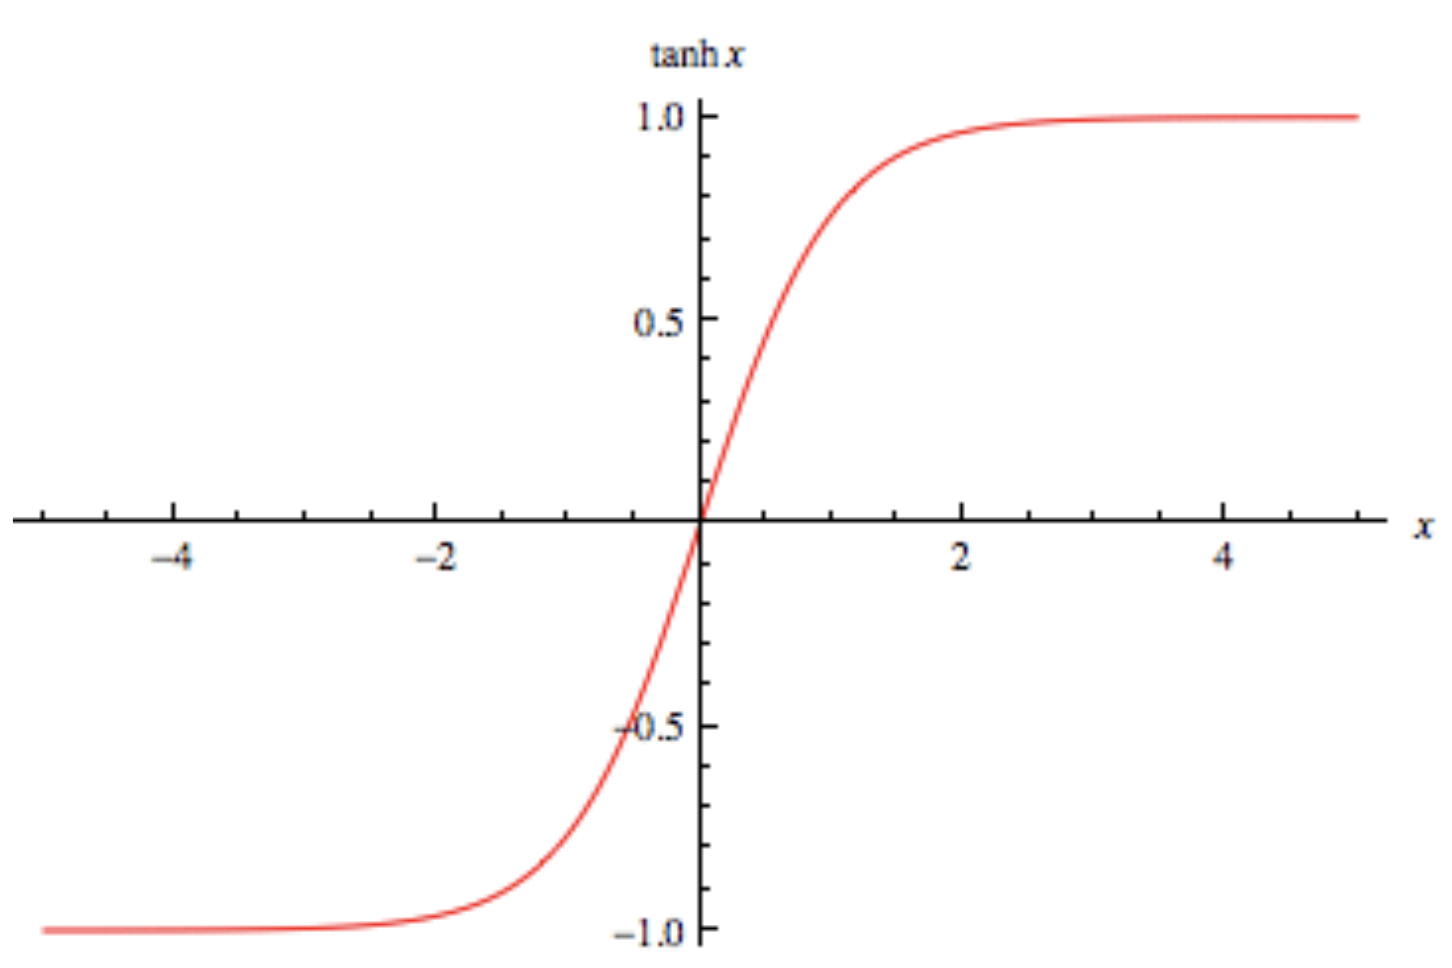
\includegraphics[width=1\textwidth]{tanh}
        \caption{Tanh activation function (from \textit{Wolfram MathWorld})}
        \label{fig:tanh}
	\end{subfigure}
	\caption{Activation functions}
\end{figure}


\subsection{Optimizers}
\paragraph{} An optimization algorithm determines the way model's learnable parameters (\textit{weights}) are updated during the training process. The aim of an optimizer is to minimize (or maximize) an objective function that is dependent on the model's weights, which is the cost function. Since the cost function is computed using the model's predictions and the latter are determined by the weights and input features, the weights have a crucial role in minimizing the cost function. The update of the model's learnable parameters takes place through \textit{backpropagation}: after the generation of the predictions, the gradient of the loss function with respect to the weights is computed; then the weights are updated in the opposite direction of the gradient (Gradient Descent). The "magnitude" of the update is given by the \textit{learning rate}, which can be decisive in the search for the loss function's global minimum. The role of an optimizer is to optimize the Gradient Descent process, in order to make it more efficient and effective.

In this project, the optimizer that has been used for all the models is Adam optimizer.

\paragraph{Adam optimizer} Adam (Adaptive Moment Estimation) is one of the most popular and used optimizers in deep learning, that usually has good performances. It is based on two intuitions: adaptive learning rate (inspired by RMSProp optimizer) and momentum optimization \cite{arXiv:adam} \cite{arXiv:optimizers}. An adaptive learning rate method computes individual learning rates for different model's learnable parameters; while a momentum method helps accelerating the Gradient Descent process by adding a fraction of the update vector of the past time step to the current update vector. This optimizer stores two moments: the first moment $m_t$ (the mean), which is estimated as the exponentially decaying average of past gradients, and the second moment $v_t$ (the uncentered variance), which is estimated as the exponentially decaying average of past squared gradients. The two moments are computed respectively as follows:
\begin{align}
    m_{t} &=\beta_{1} m_{t-1}+\left(1-\beta_{1}\right) g_{t} \\
    v_{t} &=\beta_{2} v_{t-1}+\left(1-\beta_{2}\right) g_{t}^{2}
\end{align}
where $g_{t}$ is the gradient on current mini-batch and $\beta_1$, $\beta_2$ are optimizer's decay rates, usually set close to 1. Since $m_t$ and $v_t$ are initialized as zero-vectors, they are biased towards zero, therefore they need to be corrected:
\begin{align}
    \hat{m}_{t} &=\frac{m_{t}}{1-\beta_{1}^{t}} \\
    \hat{v}_{t} &=\frac{v_{t}}{1-\beta_{2}^{t}}
\end{align}
The first moment $m_t$ is used as momentum optimization parameter, while the second moment $v_t$ is used to adapt the learning rate to each different weight. The resulting Adam update rule for model's weights is the formula:
\begin{align}
    \theta_{t+1}=\theta_{t}-\frac{\eta}{\sqrt{\hat{v}_{t}}+\epsilon} \hat{m}_{t}
\end{align}
where $\theta$ is the model weight and $\eta$ is the learning rate ($\epsilon$ is just a smoothing term usually initialized to a tiny number).

\subsection{Regularization}
\paragraph{} Regularization techniques are very useful in deep learning in order to avoid overfitting. Deep neural networks generally have a huge amount of parameters, which represent their power to learn from complex datasets; this flexibility, however, sometimes leads to the overfitting of the training set, preventing the model from making good prediction on any other dataset \cite{OReilly:handsonML}. To solve this problem, there exist several regularization methods, which in some way limit the amount of freedom of the model by adding some penalty as the model complexity increases.

The regularization techniques used in this project are the $\ell_{2}$ regularization and dropout.

\paragraph{$\mathbf{\ell_2}$ regularization} The $\ell_2$ regularization, also called Ridge Regression or Tikhonov regularization, constrains the model's flexibility by adding a regularization term to the cost function. In this way, while trying to fit the data, the model is forced to keep the weights as small as possible. The regularization term added to the loss function is the 2-norm (Euclidean distance) squared, controlled by the parameter $\lambda$, which handles the amount of regularization of the model. This is expressed by the equation:
\begin{align}
    &\textit{regularization term } = \lambda \|\theta\|_{2}^{2} = 
    \lambda \sum_{i=1}^{m} \theta_{i}^{2}\\
    &\textit{error } = (\textit{loss function}) + \lambda \sum_{i=1}^{m} \theta_{i}^{2}
\end{align}
where $\|\cdot\|_{2}$ represents the 2-norm and $m$ is the length of the weights vector $\theta$ of the model. If $\lambda = 0$, then there is no regularization, since the regularization term added to the loss function is zero. If $\lambda$ is too large, then the weights take a value very close to zero and the model underfit the data, not being able to learn from it.

\paragraph{Dropout} The dropout is probably the most popular regularization technique in deep learning. The principle is very simple: during the training process, some layer's neurons are "dropped out", which means they are set to zero and completely ignored. The neurons to shut down are selected from the input layer and the hidden layers, excluding the output neurons, and they are chosen based on a probability $p$. This means that, at each training step, each neuron has a probability $p$ of being shut down for that training step. The probability $p$ represents the dropout rate, that is the fraction of nodes to ignore.
\begin{figure}[htbp]
    \centering
    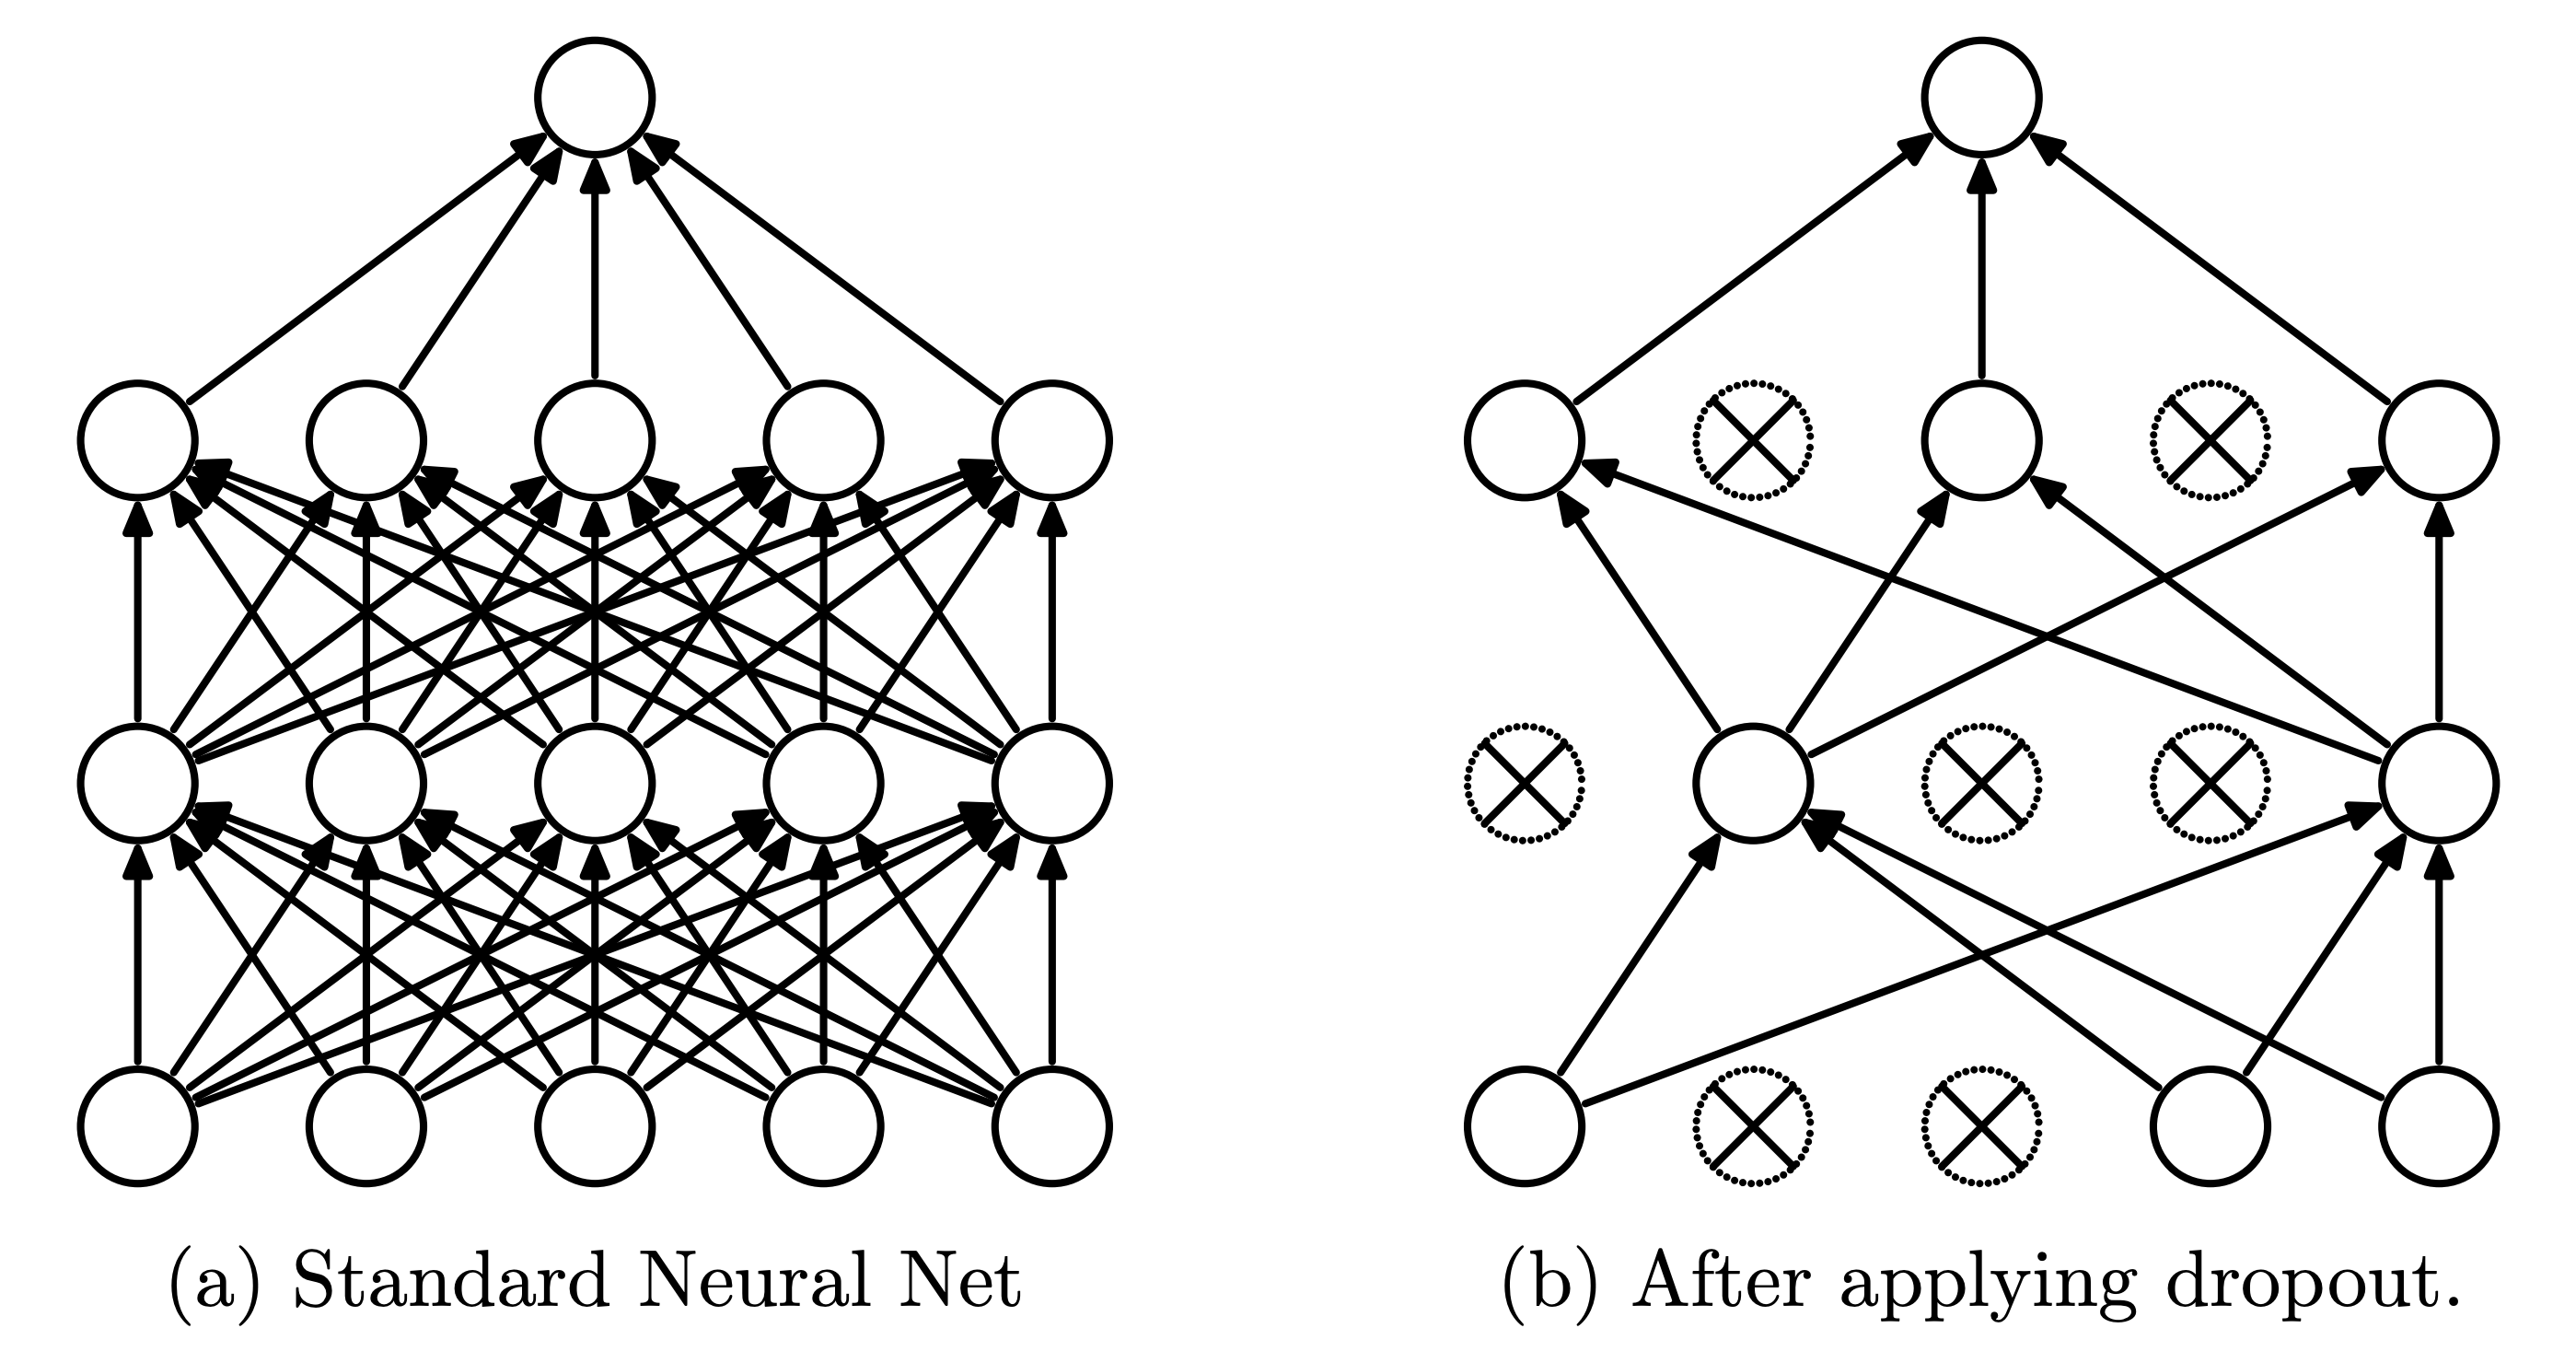
\includegraphics[width=0.7\textwidth]{dropout}
    \caption{Illustrated example of dropout (from \textit{Srivastava, Nitish, et al. ”Dropout: a simple way to prevent neural networks from overfitting”, JMLR 2014})}
    \label{fig:dropout}
\end{figure}

Figure \ref{fig:dropout} shows and example of dropout applied to a simple dense neural network. The idea behind dropout is that the network cannot rely on the features of each individual neuron, because if an essential neuron is shut down, then the network is not able to perform well. By ignoring some percentage of different neurons at each training step, the model is forced to learn more robust features, that work well together with the features of other groups of neurons. In this way, it is not dependant on the features of few individual neurons, leading to a better generalization.



\section{Classic machine learning models}
\paragraph{} Machine learning models are able to perform a specific task efficiently, without the need of explicit instructions, but relying uniquely on the patterns and features they learn from data. Giving the nature of this project's problem and the type of data we are working on, all the models that have been used have been trained in a supervised manner. This means that the training data fed to the algorithm includes the labels, that are the solutions to the problem. In the case of a classification task, the training data consist of both the data features and the respective classes of membership, so that the model can learn from examples and discover patterns that allow it to make good predictions on new data.

In this section we are going to describe the classic machine learning models that have been used, leaving the classic deep learning models (neural networks) for the next section. The models in this section are much weaker than the neural networks, but they are more efficient when the problem is simple enough to be handled by a simpler model.

\subsection{Random forest}
\paragraph{} A random forest is an ensemble of decision trees, which are machine learning algorithms able to perform both classification and regression \cite{OReilly:handsonML}. To understand how a random forest works, we first need to say a few words about decision trees.

A decision tree is a model represented as a tree in graph theory, with a root node, internal vertices, leaf nodes and edges between them. Each node can be seen as a decision unit: it contains a boolean expression based on some input features and it makes decisions based on this condition. The leaf nodes make and exception since, for classification tasks, each of them correspond to a different class. The classification of a single input instance, then, works as follows: starting from the root node, each node evaluate its boolean expression on one (or multiple) instance's feature and, depending on whether the condition is \textit{True} or \textit{False}, the path to follow continues on the left or right child of that node. The process goes on until a leaf node is reaches and the instance is finally assigned to the class corresponding to that leaf node. Figure \ref{fig:decision_tree} shows and example of a decision tree applied to the famous Iris dataset for classification. In that case, the features used by nodes to create a condition are at first the petal length and then the petal width. The three leaf nodes correspond to the tree classes: setosa, versicolor and virginica. The \textit{gini} attribute assigned to each node measures its impurity, which depends on the class distribution of the instances to which the node is applied. If $gini = 0$, then the node is pure, meaning that all the instances to which it is applied belong to the same class. If all the leaf nodes' \textit{gini} attribute is equal to zero, then the decision tree has perfectly classified all the instances.
\begin{figure}[htbp]
    \centering
    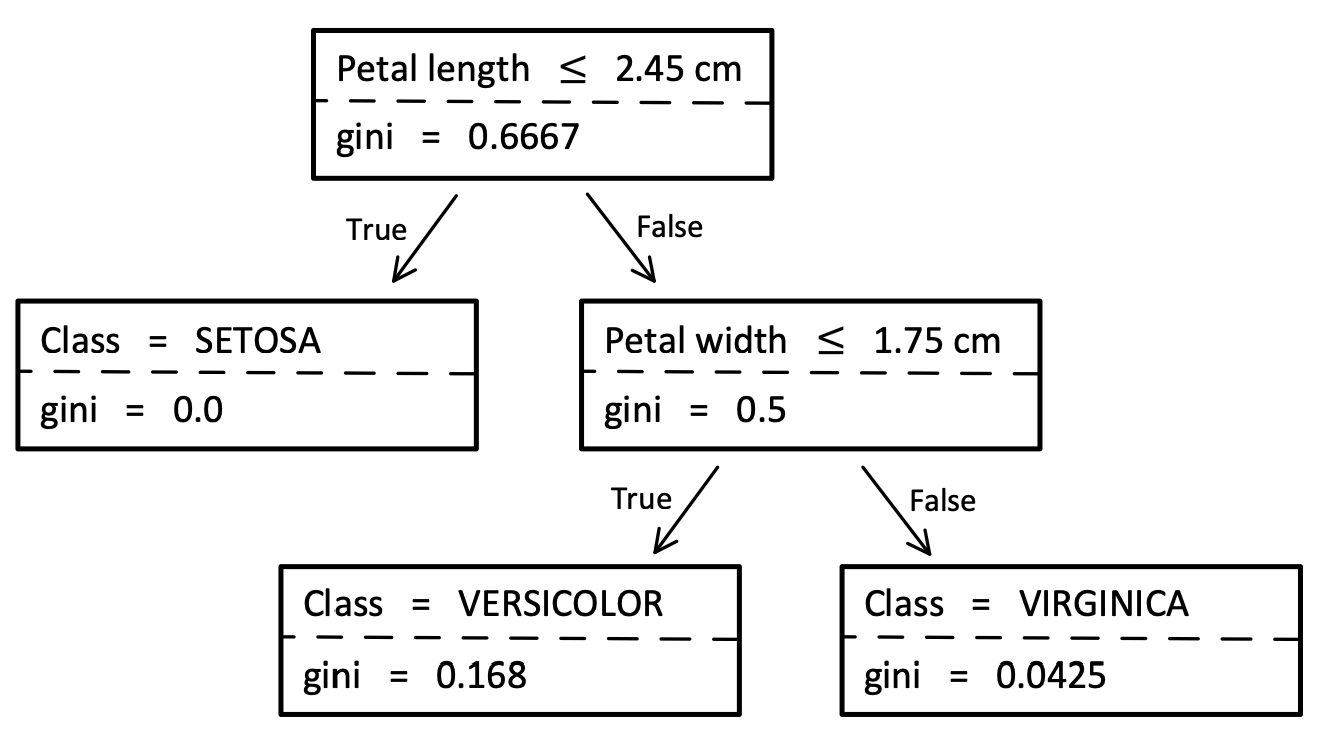
\includegraphics[width=0.7\textwidth]{decision_tree}
    \caption{Example of decision tree applied to the famous Iris dataset for classification}
    \label{fig:decision_tree}
\end{figure}

When the final prediction is computed using an ensemble of decision trees, we talk about random forest. In a random forest, $k$ different decision trees are trained in parallel on different random subsets of the training set. The sampling of the data can be performed with replacement (\textit{bootstrapping}), like in this project, or without replacement. Both methods allow training instances to be selected multiple times for different decision trees, but, when using bootstrapping, the same instance could be selected multiple times also for the same decision tree. Once all the decision trees have been trained, the random forest prediction is computed by aggregating the predictions of all its decision trees. Typically the statistical mode is used as aggregation function, but the average can be used as well. A random forest can be regularized by setting the number of decision trees to use and their maximum depth.

In general, random forest algorithms work better than decision trees and are less prone to overfitting. The reason is the greater tree diversity: in addiction to the data sampling, when splitting a node during the construction of the tree, the split is chosen no longer as the best among all features, but as the best among a random subset of the features.

\subsection{Gradient boosting}
\paragraph{} Gradient boosting (tree-based) is very similar to random forest, as it is itself an ensemble of decision trees. Differently from random forest, in gradient boosting the decision trees are trained in a sequential way, one at a time, and each one tries to correct the errors made by its predecessor. In particular, each new decision tree is fitted on the residual errors made by the previous one. Therefore, while the first decision tree of the sequence will fit the instances $\mathbf{X}$ and the targets $\mathbf{y}$, the second decision tree will fit $\mathbf{X}$ and the residual errors $y_1 = \mathbf{y} - \hat{y}_1$, where $\hat{y}_1$ are the predictions made by the first decision tree on $\mathbf{X}$. Likewise, the third decision tree will fit $\mathbf{X}$ and the residual errors $y_2 = y_1 - \hat{y}_2$, where $\hat{y}_2$ are the predictions made by the second decision tree on $\mathbf{X}$, and so on. So we can consider gradient boosting as a gradient descent algorithm.

Usually gradient boosting have better performance with respect to random forest, but, since decision trees are not trained independently, it is more prone to overfitting.

\subsection{Support vector machine}
\paragraph{} SVM (Support Vector Machine) is a very powerful machine learning algorithm able to perform both linear and non-linear classification and regression \cite{OReilly:handsonML}. It is a binary classifier, but it can be used also as a multiple-class classifier through some trick. In order to classify data, the SVM represents the instances as points on a decision surface and divides them through a decision boundary that is placed in the middle of the largest possible gap between the two classes' instances (positive and negative class). In other words, if we imagine the data projected in a 2-dimensional space, the SVM tries to find a line able to separate the positive and negative instances staying as far away as possible from the closest instances. This situation is illustrated in Figure \ref{fig:svm_line}, where the two group of instances, belonging to the blue and green classes, are divided by the red line. The boundary generated by the SVM is placed as far as possible from the instances, trying to maximize the distance $w$ from the nearest instances. In this way, in case we made a small error in the location of the boundary, we have a margin of error that prevents a misclassification. The instances that lie on the edges of the decision boundary's margins are called \textit{support vectors} (in Figure \ref{fig:svm_line} they are represented as filled circles). The position of the support vectors completely determine the max-margin decision boundary and the distance between support vectors of different classes determine the width of the optimal boundary’s margins.
\begin{figure}[htbp]
    \centering
    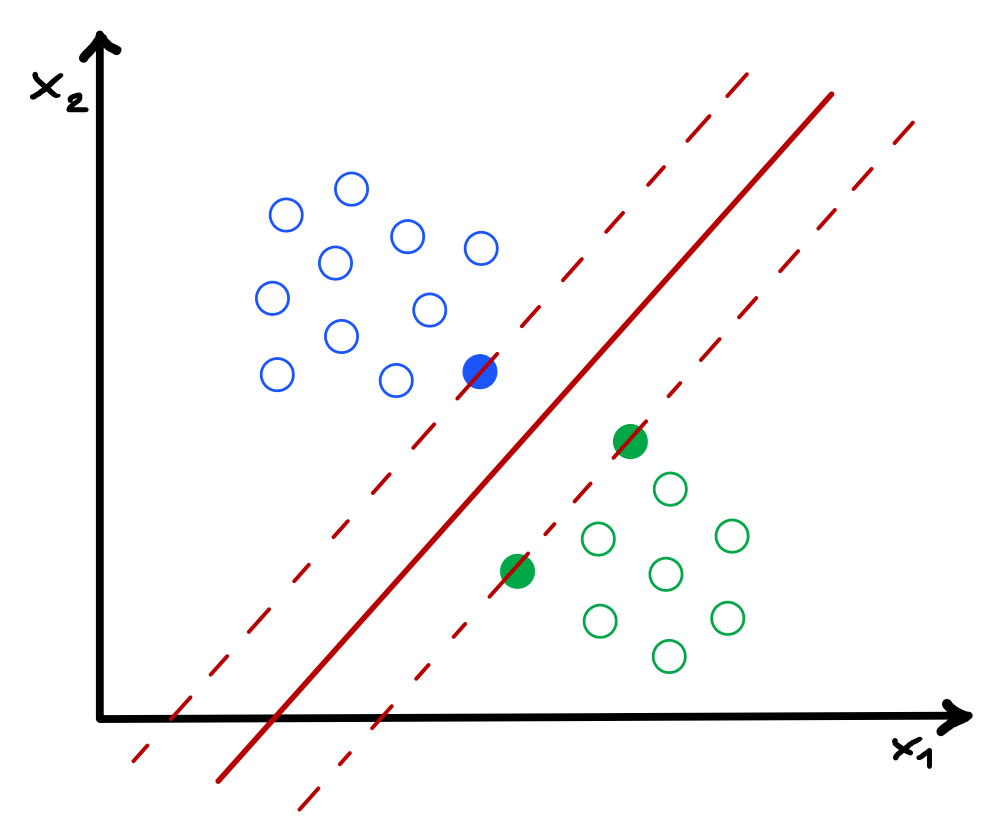
\includegraphics[width=0.4\textwidth]{svm_line}
    \caption{Example of SVM decision boundary for data classification}
    \label{fig:svm_line}
\end{figure}

In SVMs, the data are projected to a $d$-dimensional space, where $d$ is the number of data features, and the decision boundary that classifies the data is a hyperplane. A hyperplane is a subspace of an ambient space that is one dimension less than the ambient space: for example, if a space is 2-dimensional, then its hyperplanes will be 1-dimensional (lines). In general, if the ambient space is n-dimensional, its hyperplanes will be (n-1)-dimensional. In SVMs context, an hyperplane is the subspace of the decision space that the SVM constructs in such a way that the margin of separation between the two classes' instances is maximized.

If the data points are linearly separable, the SVM is able to construct two parallel hyperplanes that separate the data points in the two respective classes. The hyperplanes can be respectively described by the two equations:
\begin{align}
    &\vec{w} \cdot \vec{x}^{+}-b=1 \\
    &\vec{w} \cdot \vec{x}^{-}-b=-1
\end{align}
The distance between the two hyperplane is $\frac{2}{\|\vec{w}\|}$, so, in order to maximize the distance between them, we want to minimize $\|\vec{w}\|$, while avoiding margin violation (\textit{hard margin}) or limiting them (\textit{soft margin}).

Hard margin can be used for linear problems, where the data points are linearly separable. In this case, the max-margin hyperplane is completely determined by those data points which are nearest to it and we want to prevent data points from falling into the margin. To reach this result, we can use the following objective function, subjected to the following constraints:
\begin{align}
    &\text{objective function }= \min \frac{1}{2}\|\vec{w}\|^2 =  \min \frac{1}{2} w^{T} w\\
    &\text{constraints }= \left\{\begin{array}{ll}{\text{if } y=1 :} & {w^{T} x+b \geq 1} \\ {\text{if } y=0 :} & {w^{T} x+b <-1}\end{array}\right.
\end{align}
These constraints guarantee that each point lies on the correct side of the margin.

In some cases, the problem can be non-linear and therefore not solvable with hard-margin; in other cases, the problem can be linear, but we would like a general solution that takes into account the presence of some errors in the data. In these situations, soft-margin can be used in place of hard-margin. Soft-margin SVMs allow some exceptional data points to fall into the margin or to lie on the wrong side of the margin. Soft-margin SVM introduces two new parameters: $\varepsilon_i$ represents the distance of $x_i$ from his real class margin hyperplane; $C$ is a parameter that allows to control better the softness of the margin, defining the tradeoff between the objective and the constraints. If $C$ is very big, the SVM becomes very rigid and behaves similarly to hard-margin; on the other hand, if $C$ is very small, the SVM allows a lot of errors. Soft-margin is defined by the following objective function, subjected to the following constraints:
\begin{align}
    &\text{objective function }= \min \frac{1}{2} w^{T} w + C \sum^{n}_{i=1} \varepsilon_i\\
    &\text{constraints }= \left\{\begin{array}{lll}{\text{if } y=1 :} & {w^{T} x+b \geq (1 - \varepsilon_i)} \\ {\text{if } y=0 :} & {w^{T} x+b < (-1 + \varepsilon_i)} \\ {\text{for all } i :} & {\varepsilon_i \geq 0}\end{array}\right.
\end{align}
Figure \ref{fig:svm_formulas} shows a geometric representation of the parameters and formulas just presented.
\begin{figure}[htbp]
    \centering
    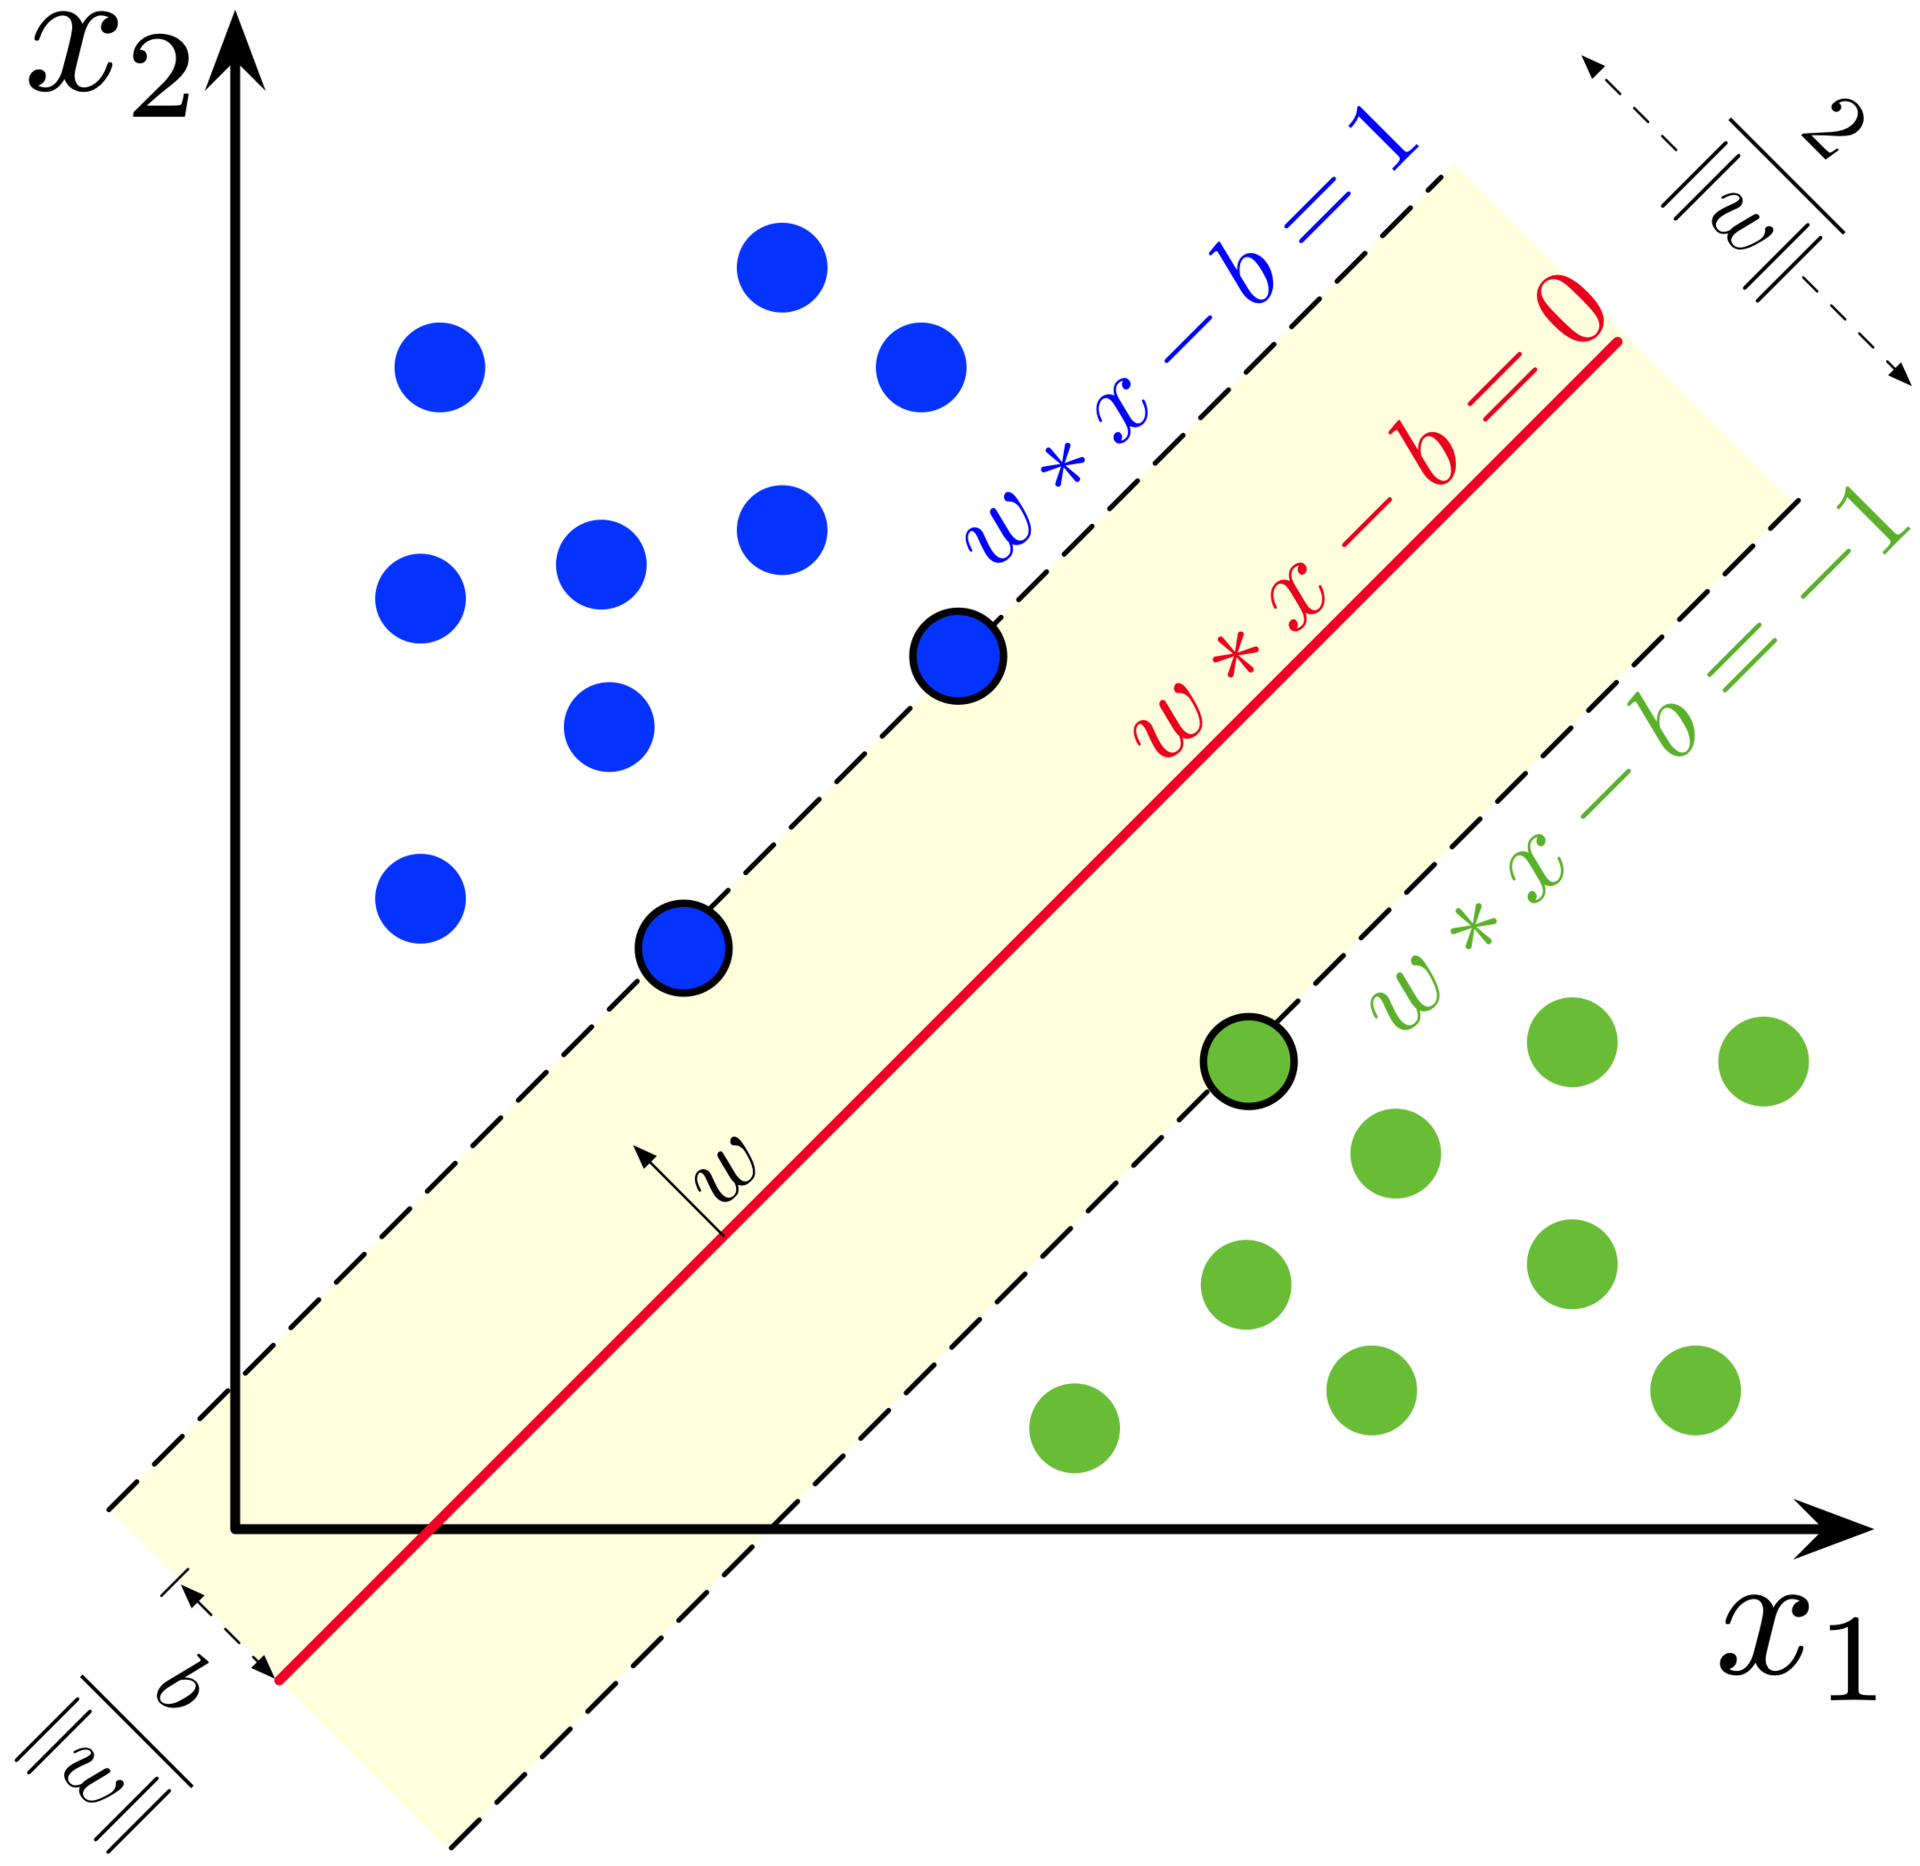
\includegraphics[width=0.4\textwidth]{svm_formulas}
    \caption{Geometric representation of SVM's equations}
    \label{fig:svm_formulas}
\end{figure}

When data are not linearly separable, we can still use SVM in two ways: we can simply use soft-margin and permit some tolerance in presence of errors, or we can rely on a kernel function $K(a, b)$. A kernel function allows the SVM to lead the data points to a situation where they are linearly separable again. Indeed, the data can be mapped to a higher-dimensional feature space, where they are linearly separable by an optimal hyperplane. A feature map is the function that maps the data points to an higher-dimensional feature space: the function $\phi(x_i)$ maps every $x_i$ to the new feature space:
\begin{align}
    <\phi(a), \phi(b)>
\end{align}
The increase of space's dimensions can be computationally expensive, due to the computation of all the additional features. To avoid an high-cost computation, we can use the \textit{kernel trick}: applying a kernel function allows to compute the dot product of weights in the lower-dimensional space instead of in the higher-dimensional space:
\begin{align}
    <\phi(a), \phi(b)> = K(a, b)
\end{align}
The trick consists in expressing the problem just in function of the dot products, without the need to know the entire mapping to the new feature space. Actually, a kernel is a function that is able to compute the dot product $\phi(a)^T \phi(b)$ based only on the original vectors $a$ and $b$, without the need to compute the transformation $\phi$ on the vectors. Figure \ref{fig:svm_nonlinear} shows an example of a non-linear separable problem that could be solved by mapping data to a higher-dimensional space.
\begin{figure}[htbp]
    \centering
    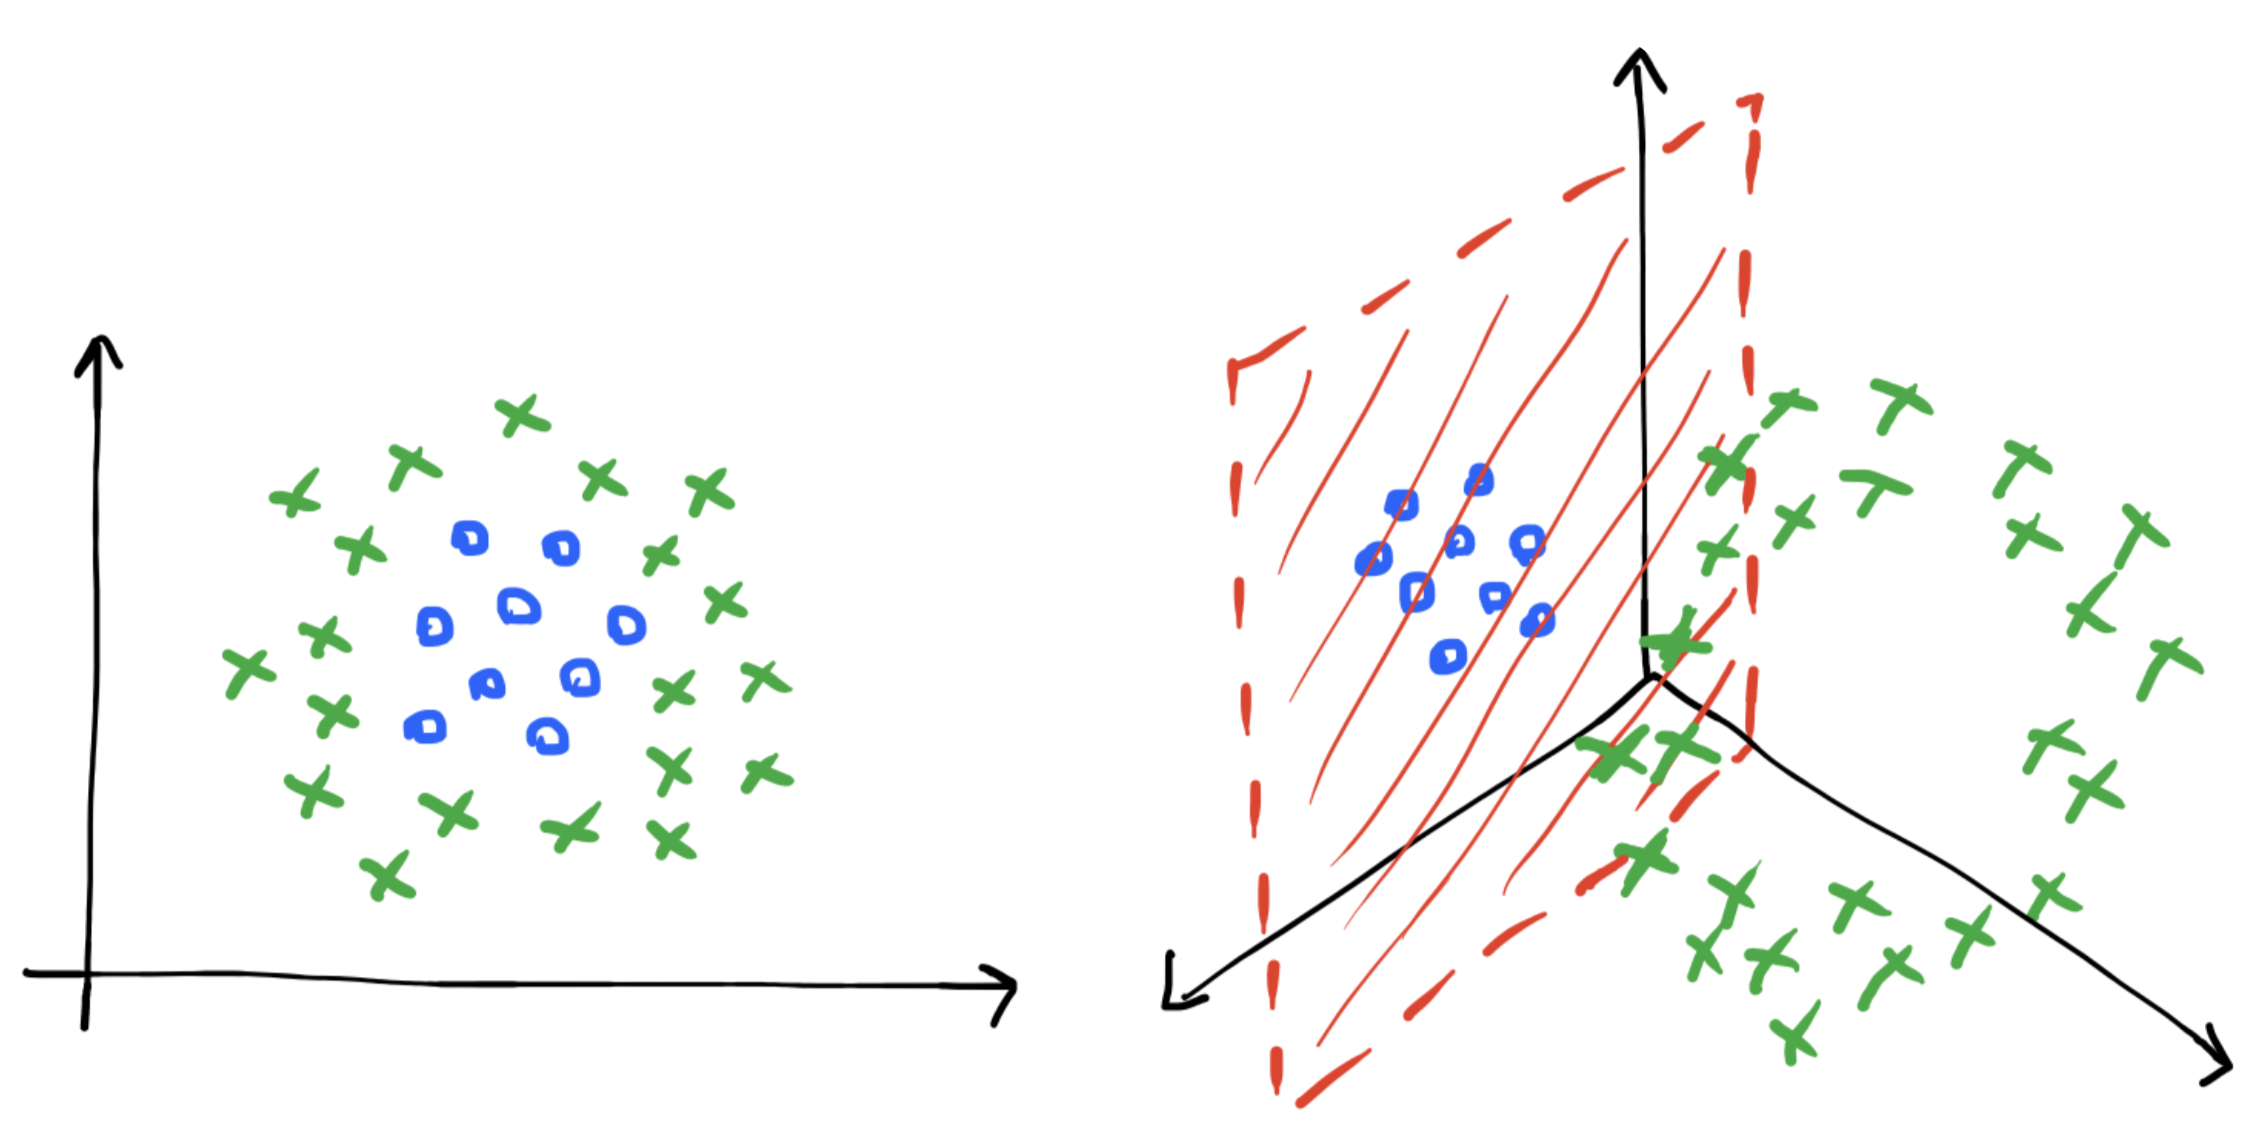
\includegraphics[width=0.6\textwidth]{svm_nonlinear}
    \caption{Example of a non-linear separable problem solved in a higher-dimensional space}
    \label{fig:svm_nonlinear}
\end{figure}

A frequently used kernel is the Gaussian RBF kernel (Radial Basis Function kernel). This kernel generates new features by measuring the distance between the support vectors and all other instances: the function value decreases as the distance from the support vectors grows, so it can be considered a similarity measure. Through Gaussian RBF kernel, the input vector is mapped to an infinite vector and then normalized by dividing each component by the vector’s length. The Gaussian RBF kernel is defined by the equation:
\begin{align}
    K(a, b) = \exp \left(-\frac{\|a - b\|^{2}}{2 \sigma^{2}}\right) = \exp \left( -\gamma \|a - b\|^{2} \right)
\end{align}
The hyperparameter $\gamma = \frac{1}{2 \sigma^{2}}$ can be used as regularization term, since it controls how strict the decision boundary is by determining a strong sharpness if $\gamma$ is big (if $\sigma$ is small) and a weak sharpness otherwise (if $\sigma$ is big). So if the SVM is overfitting, $\gamma$ should be reduced, and if it is underfitting, $\gamma$ should be increased.

The kernel trick can be used together with the soft-margin in order to reach good performance and better generalization.

\section{Classic deep learning models}
\paragraph{} Deep learning is a subfield of machine learning that differentiate itself for the specific type of models that it uses in order to learn a certain task. These models are \textit{artificial neural networks}.

Artificial neural networks are very powerful and versatile models that are inspired by human neural networks: the structure of artificial neural networks is comparable to the one of our brain, which has neurons and connection between them to transmit electrical impulses. Similarly, artificial neural networks is composed by several neurons which are the computational cores of the model and which transmit the processed information to each other.

Artificial neural networks (or simply neural networks) organize the neurons in layers: the input layer is represented by the input data, the output layer is the last one that process data and returns the result of the entire model, while all the layers in between are called \textit{hidden layers} and, in addition to transforming the data, they send the processed information to the next layer. Figure \ref{fig:nn_layers} shows an example of a typical network's structure.
\begin{figure}[htbp]
    \centering
    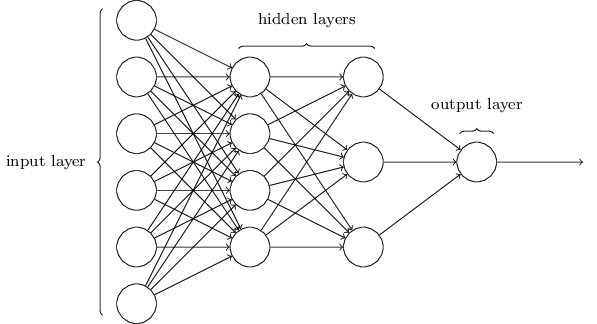
\includegraphics[width=0.7\textwidth]{nn_layers}
    \caption{Neural network's structure and layers (from \textit{Neural Networks and Deep Learning} free online book)}
    \label{fig:nn_layers}
\end{figure}
Each neuron processes the input data by computing a linear transformation, that is the weighted sum $\sum$ plus a bias, followed by a non-linear transformation, that is the activation function $\sigma$. The weighted sum is performed by multiplying each input feature $x_i$ for its corespondent weight $w_i$ and then taking the sum of all the resulting products. A bias term $b = 1$ is added to the weighted sum to help the network approximating the objective function. The result of this linear transformation represents the input of the activation function, which, as already mentioned, introduces the non-linearity properties by mapping the data to the desired output. Figure \ref{fig:nn_neuron} illustrates the functioning of a single neuron. 
\begin{figure}[htbp]
    \centering
    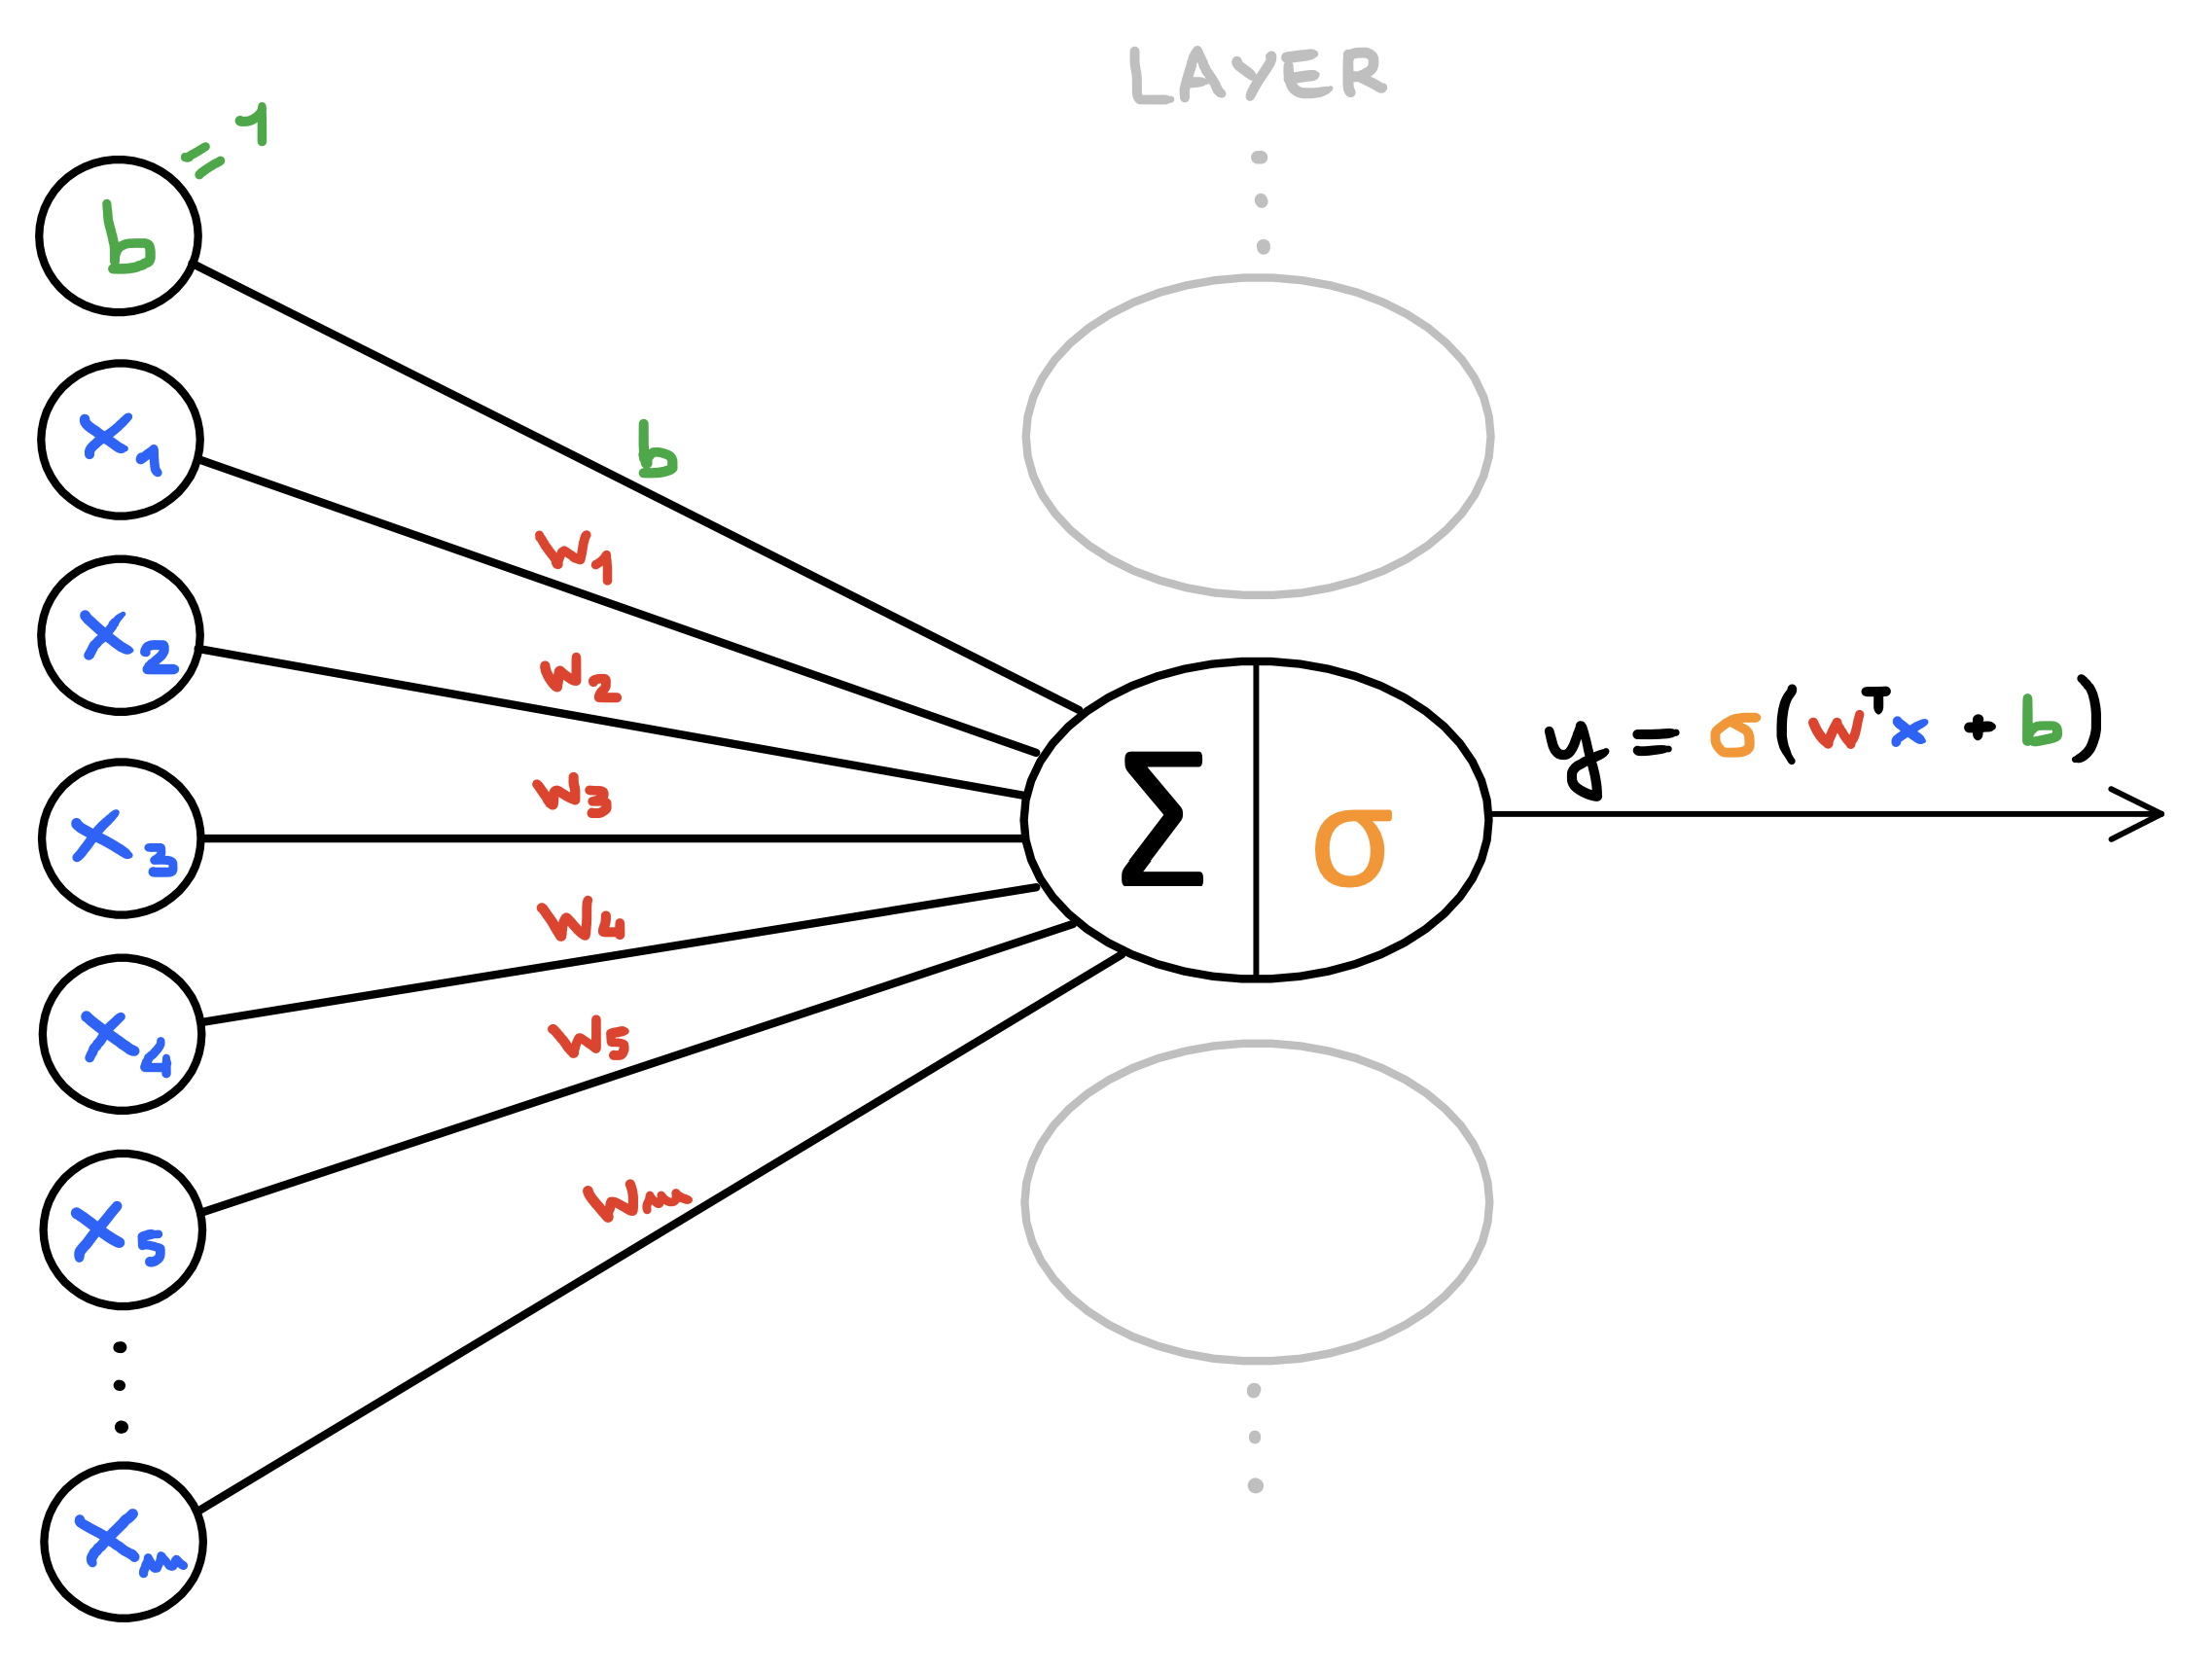
\includegraphics[width=0.6\textwidth]{nn_neuron}
    \caption{Illustrated description of the functioning of a single neuron}
    \label{fig:nn_neuron}
\end{figure}
Each neuron in a layer performs these operation and the outputs of all the neurons of that layer will be the inputs for the next layer. Formally, the inputs and outputs of layers of a neural network can be described by the equations:
\begin{align}
    &h^{\textit{out}}_{0} = \mathbf{X}\qquad\qquad\qquad \text{(input layer)}\\
    &h^{\textit{in}}_{i} = h^{\textit{out}}_{i-1} \times \mathbf{W}_i + \mathbf{B}_i\\
    &h^{\textit{out}}_{i} = \phi_i (h^{\textit{in}}_{i})
\end{align}
where $\mathbf{X}$ is the features matrix of input data, $\mathbf{W}_i$ is the weights matrix of layer $i$, $\mathbf{B}_i$ is the bias vector of layer $i$, $\phi_i$ is the activation function used by neurons of layer $i$, and the operator $\times$ represents matrix multiplication.

\subsection{Dense neural network}
\paragraph{} A dense neural network (or fully-connected neural network) is a network that consists of a sequence of fully-connected layers \cite{OReilly:TFforDL}. Each layer represents a function (linear and non-linear transformations) from $\mathbb{R}^F$ to $\mathbb{R}^{F_m}$. This means that, for each input instance having $F$ features, the corresponding output will have dimensionality $F_m$, where $F_m$ is the number of neurons in the network's output layer (the $m$-th layer). Even for the hidden layers, the output dimension depends on the number of neurons present in the layer.

The network is called \textit{fully-connected} because the output of each neuron in one layer is sent as input of each neuron in the next layer, so there is a direct connection between all the neurons belonging to subsequent layers. Figure \ref{fig:nn_dense} shows and example of dense neural network, making visible the full interconnection between subsequent layers.
\begin{figure}[htbp]
    \centering
    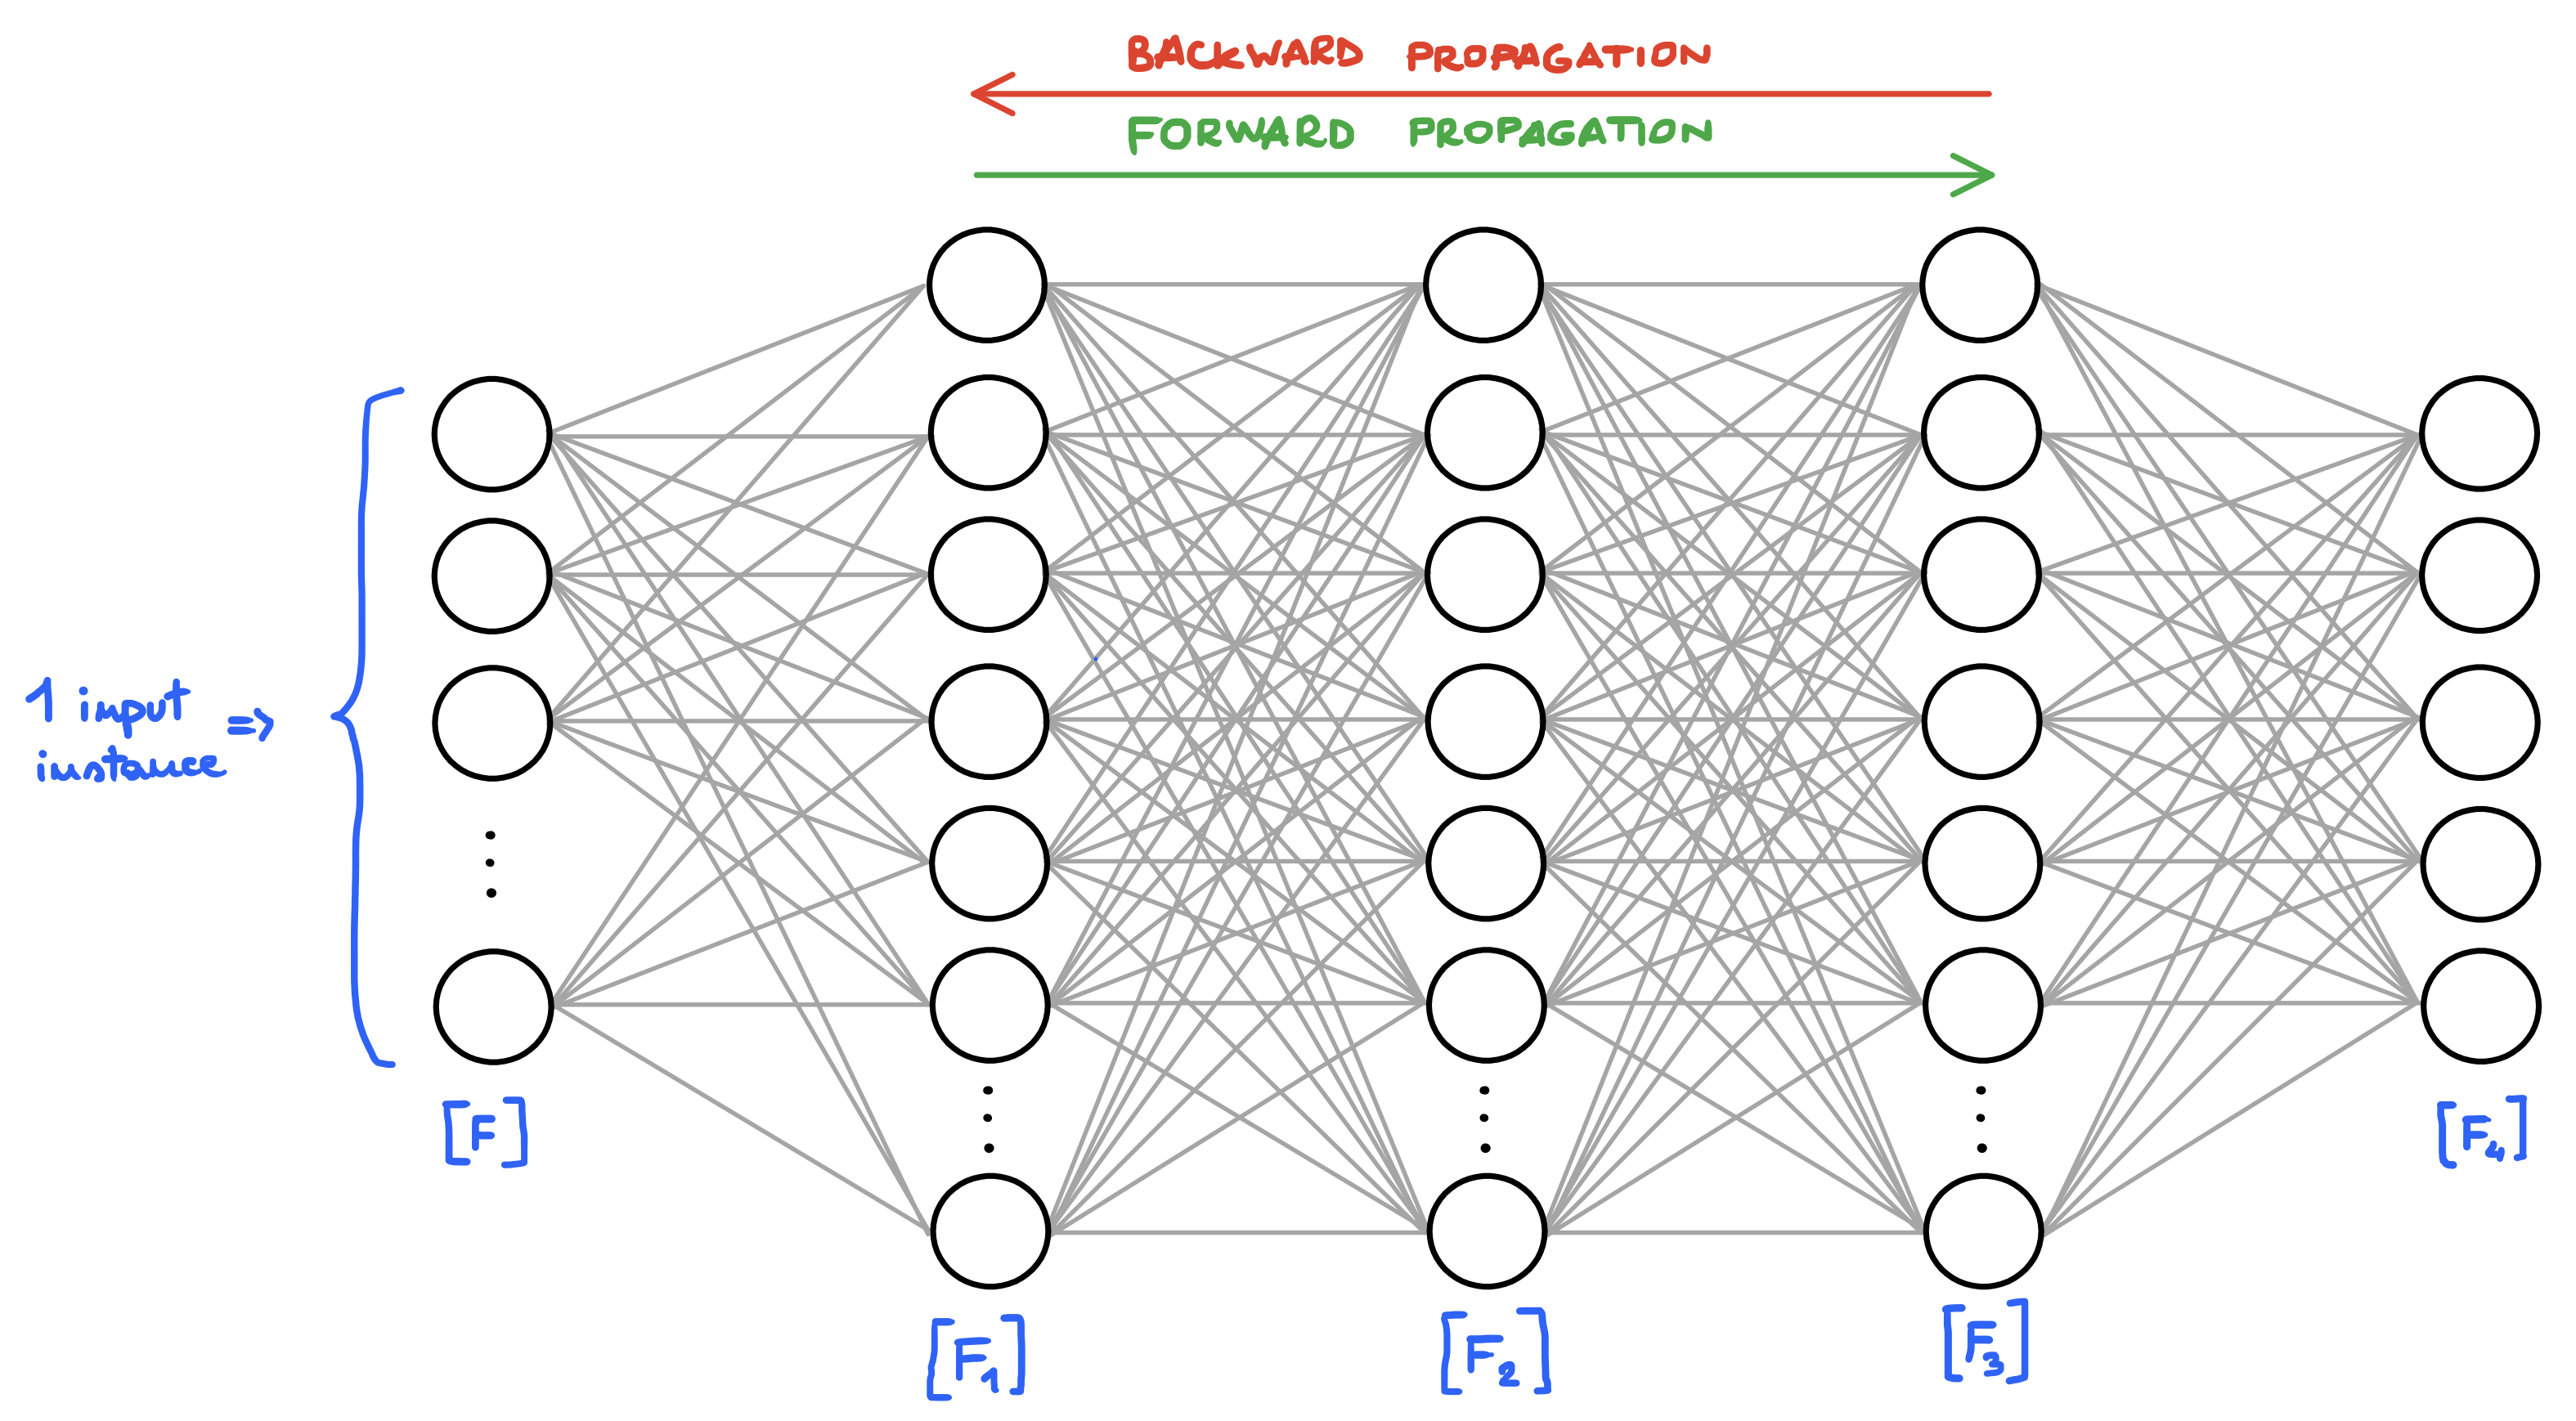
\includegraphics[width=0.9\textwidth]{nn_dense}
    \caption{Example of dense neural network}
    \label{fig:nn_dense}
\end{figure}

For each training input instance, the model computes the output of every neuron in each consecutive layer until it reaches the final predictions from the output layer (\textit{forward pass)}. After that, it compares its prediction with the actual targets and measures the output error. The error is then propagated through each layer in reverse in order to compute the error contribution (error gradient) from each neuron's connection, until it reaches the input layer (\textit{backward pass}). The error is then used by the optimizer to update the connections weights and allow the model to learn. Dense neural networks are included in the category of feed-forward neural networks, since the activation flows only in one direction.

When used for classification tasks, the output layer of a dense neural network has a number of neurons that is equal to the number of classes of the data. In this way, each output of the network (computed through softmax or sigmoid activation function) corresponds to the estimated probability that the input instance belongs to the corresponding class. The instance is then assigned to the class which obtained higher probability.

\subsection{LSTM neural network}
\paragraph{} LSTM neural networks are a special case of a more general category, which is the recurrent neural networks \cite{OReilly:handsonML}; therefore we are going to first present the basics of recurrent neural networks and then explore LSTM neural networks.

Recurrent neural networks (RNN) are usually used to analyze sequences of data and time series in order to predict the future, thanks to their ability to "memorize" past information. This is due to the fact that they are not feed-forward network, since the output of a neuron is sent back to itself. In other words, at each time step $t$, a recurrent neuron receives the features of the input $x_t$ as well as its own output $y_{t-1}$ from the previous time step. In this way, each input of a recurrent neuron is determined by the current input instance alongside with some information from all the previous instances. Expanding this logic to an entire layer of recurrent neurons, at each time step $t$, each neuron receives both the input $x_t$ as well as the entire layer's output $y_{t-1}$ from the previous time step. Figure \ref{fig:nn_recurrent} illustrates the logic behind a recurrent neural network, showing the network unrolled through time.
\begin{figure}[htbp]
    \centering
    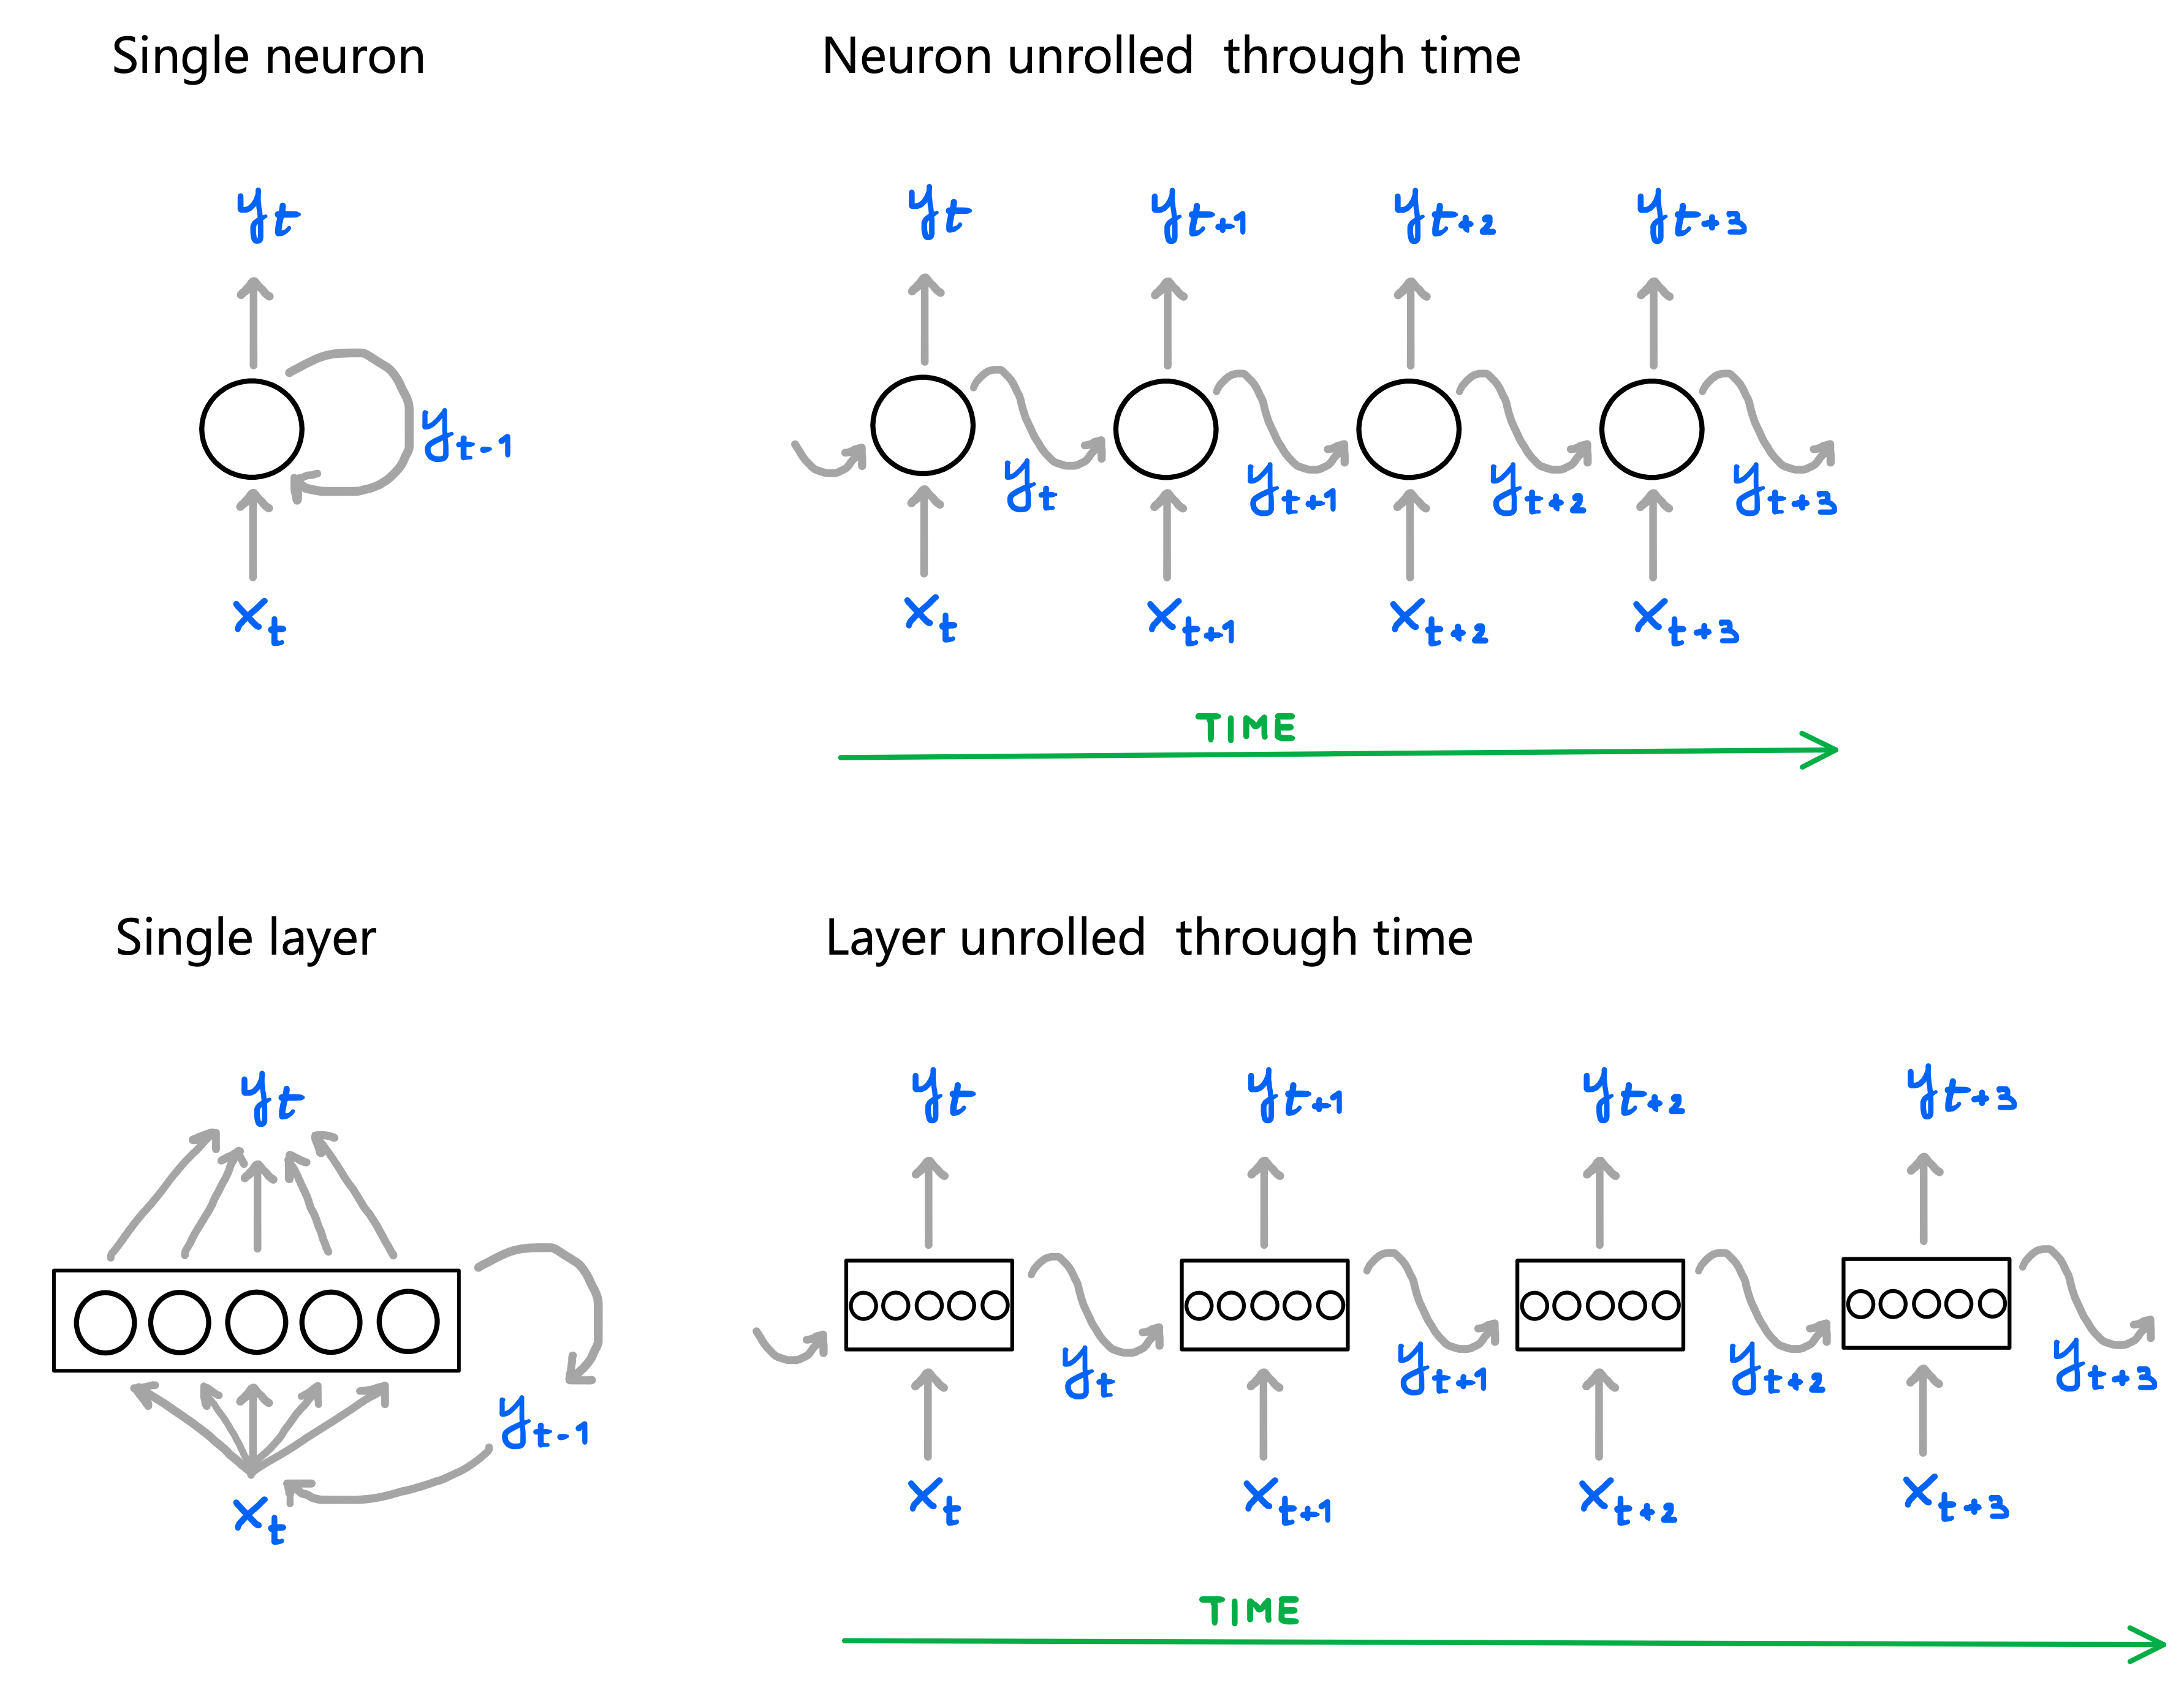
\includegraphics[width=1\textwidth]{nn_recurrent}
    \caption{Logic behind a recurrent neural network}
    \label{fig:nn_recurrent}
\end{figure}

Each recurrent neuron has two sets of weights, one for the inputs $x_t$ and the other for the previous output $y_{t-1}$. Naming $\mathbf{W}_x$ and $\mathbf{W}_y$ respectively these two sets of weights, we can rewrite the equation for the output $\mathbf{Y}_t$ of a recurrent layer:
\begin{align}
    \mathbf{Y}_t = \phi (\mathbf{X}_t \mathbf{W}_x + \mathbf{Y}_{t-1} \mathbf{W}_y + \mathbf{b})
\end{align}
where $\phi$ is the activation function of the layer and $\mathbf{b}$ is the bias. Concatenating the inputs $[\begin{array}{ll}{\mathbf{X}_t} & {\mathbf{Y}_{t-1}}\end{array}]$ and the weights $\mathbf{W} = \left[\begin{array}{c}{\mathbf{W}_x} \\ {\mathbf{W}_y}\end{array}\right]$, we can rewrite the equation as:
    \begin{align}
        \mathbf{Y}_t = \phi ([\begin{array}{ll}{\mathbf{X}_t} & {\mathbf{Y}_{t-1}}\end{array}] \mathbf{W} + \mathbf{b})
    \end{align}

It should be clear by now that each output at time step $t$ is a function of the inputs from all the previous time steps. For this reason, we can say that the network is able to store some sort of "memory" of the past inputs and to use this information for the outputs of the the following time steps. A neuron, or layer of neurons, that is able to preserve some state across time steps is called a \textit{memory cell}. A cell's state at time $t$ can be denoted with $\mathbf{h}_t$, which corresponds to a function $\mathbf{h}_t = f(\mathbf{h}_{t-1}, \mathbf{x}_t)$. In the case of basic memory cells like the ones in a recurrent neural network, the element $\mathbf{h}_{t-1}$ corresponds exactly to the notation $\mathbf{y}_{t-1}$ that we used until now to denote the output from the previous time step.

The classic recurrent neural network model presents some drawbacks. First of all, when the network is trained on long sequences, it may suffer form the vanishing/exploding gradient problem, taking forever to train. Moreover, on the long run, the memory of information about the first time steps tends to fade away, since part of the information is lost at each step. We could consider the RNN to have a short-term memory, which is not optimal when we need to predict events based on a long sequence of time steps. That is where the LSTM neural network comes in.

An LSTM neural network, differently from a RNN, is made of \textit{Long Short-Term Memory} (LSTM) cells \cite{NeuralComputation:lstm}. This type of cells allows the model to perform much better and to converge faster, in addition to preserving long-term information in long sequences. As shown in Figure \ref{fig:rnn_vs_lstm}, while the standard RNN cell contains only a single layer, the LSTM cell contains four interacting layers, each one having a well-defined purpose.

\begin{figure}[htbp]
    \centering
    \begin{subfigure}[t]{0.8\textwidth}
		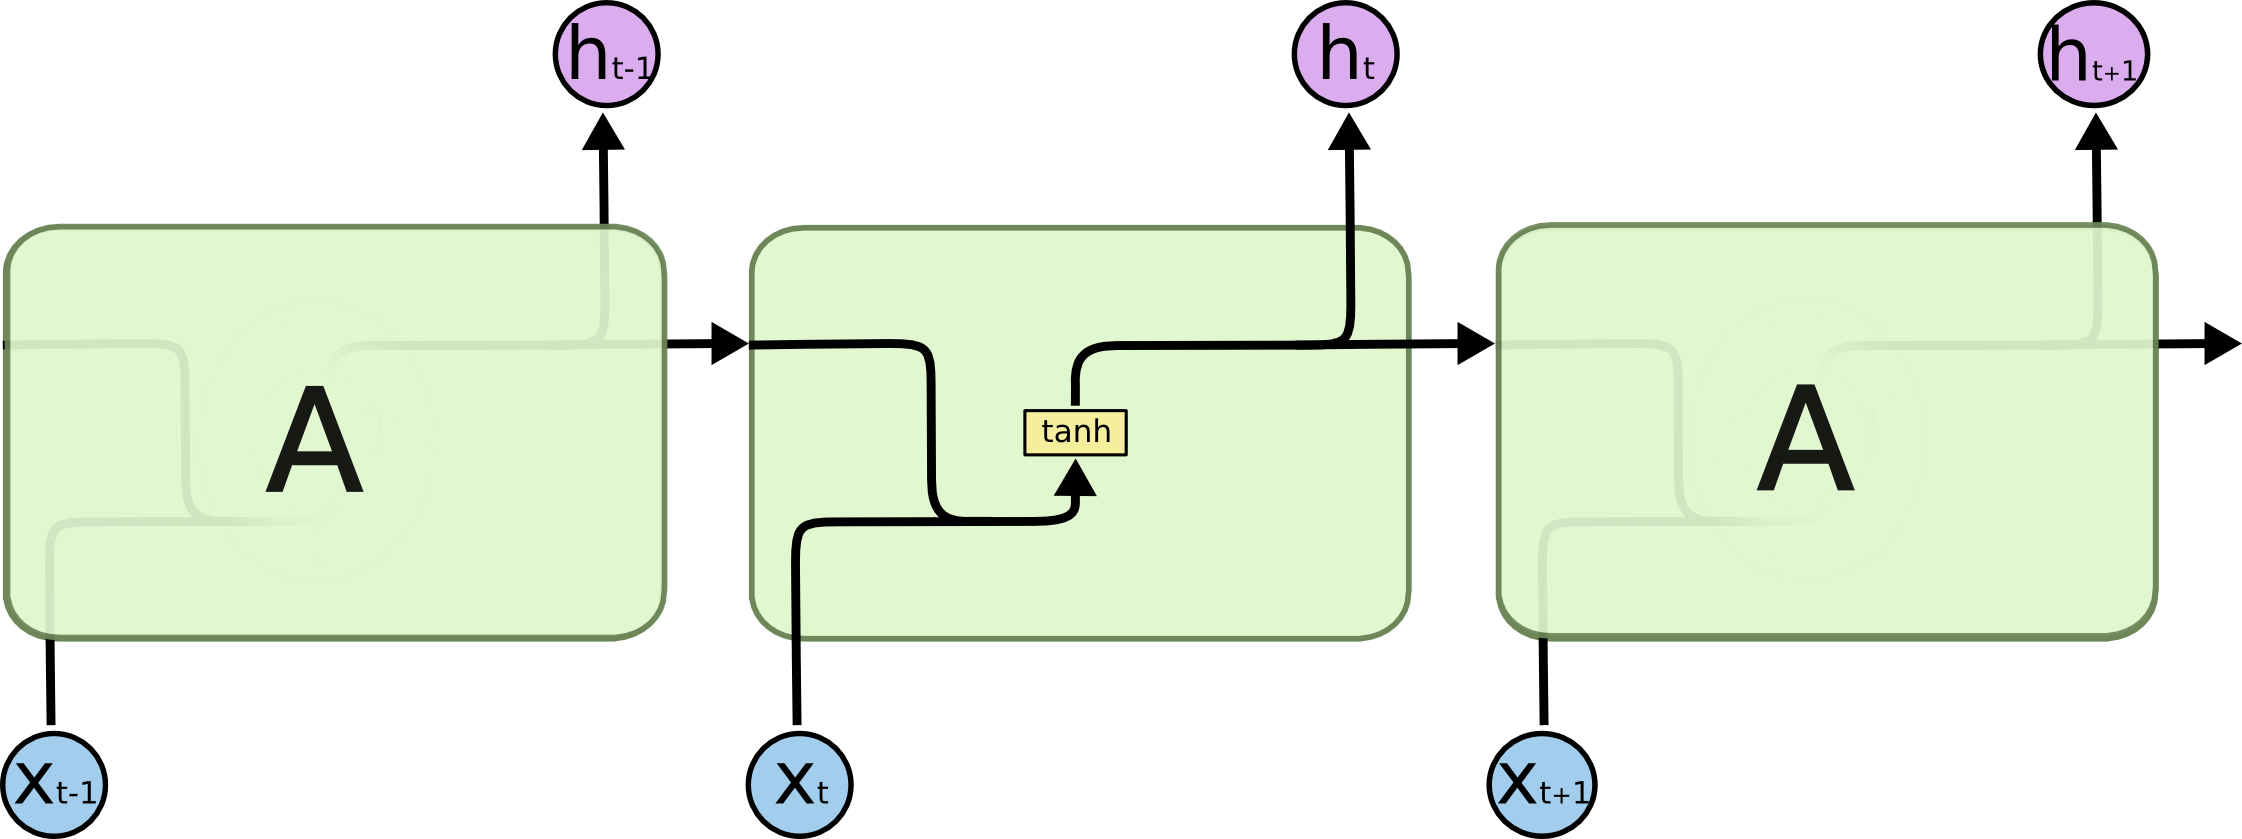
\includegraphics[width=1\textwidth]{nn_simplernn}
        \caption{Standard RNN cell}
        \label{fig:nn_simplernn}
	\end{subfigure}
	~
	\begin{subfigure}[t]{0.8\textwidth}
		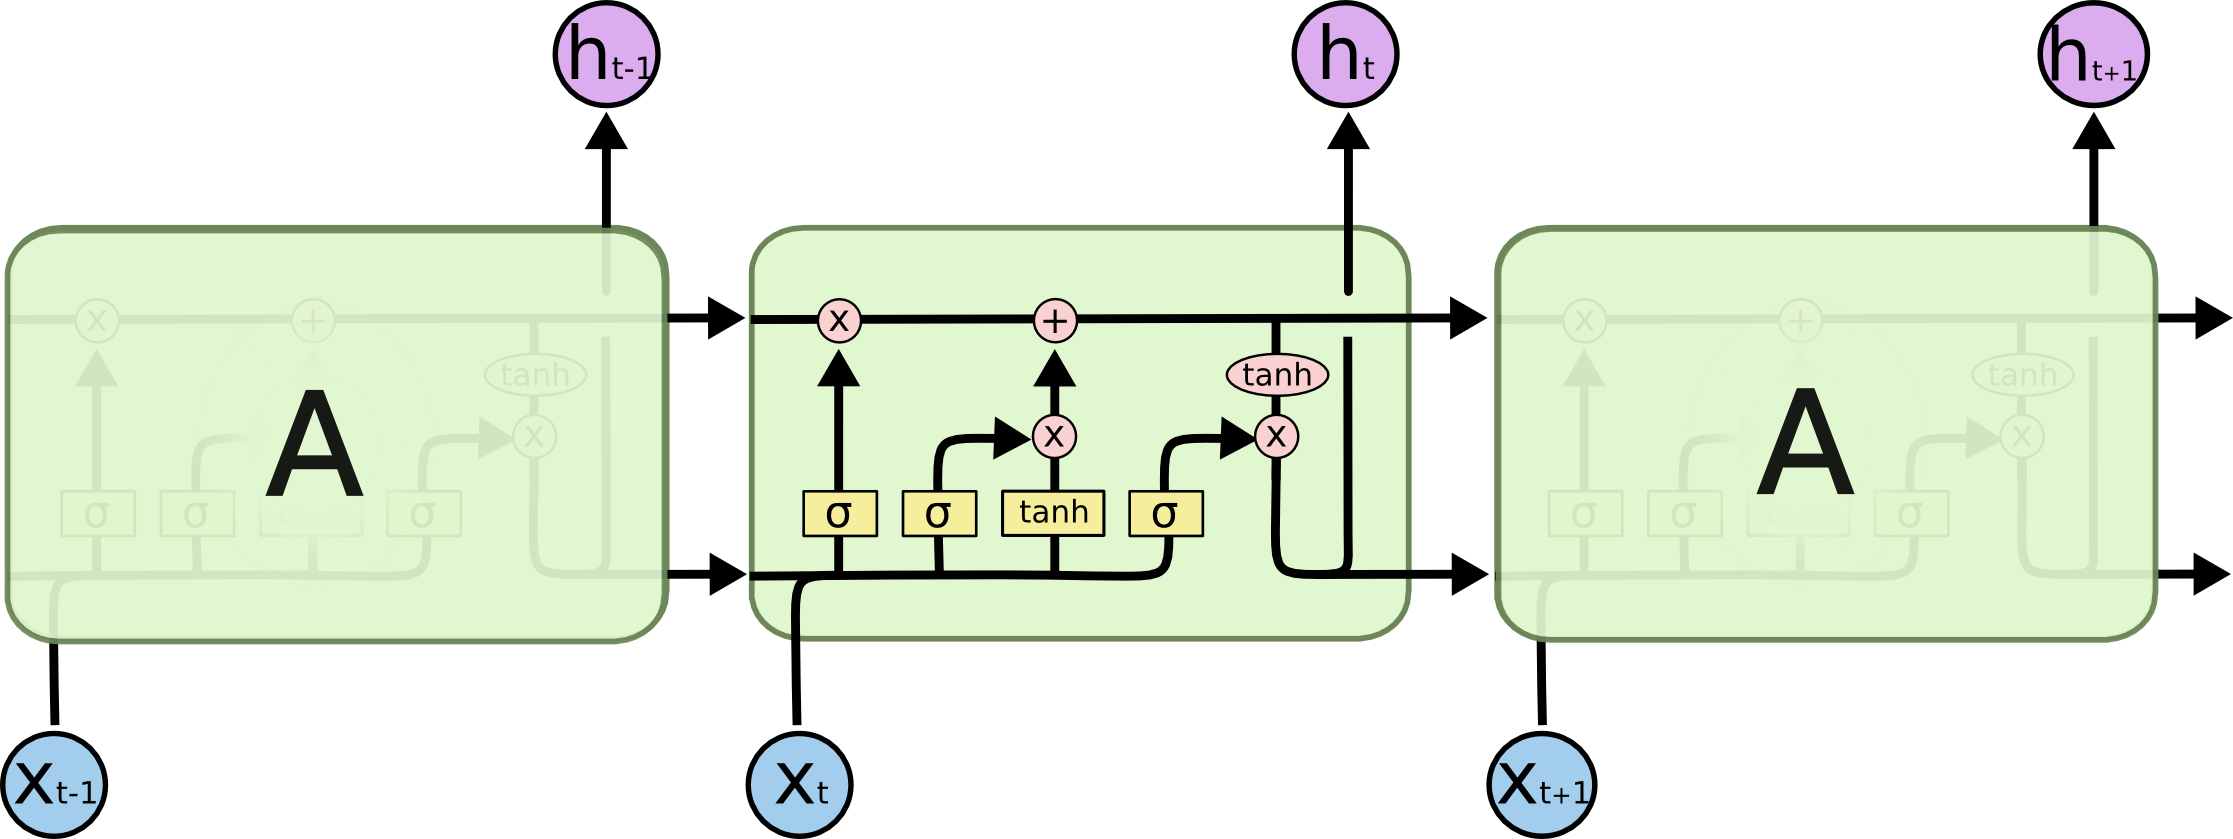
\includegraphics[width=1\textwidth]{nn_lstm}
        \caption{LSTM cell}
        \label{fig:nn_lstm}
    \end{subfigure}
    ~
    \begin{subfigure}[t]{0.6\textwidth}
		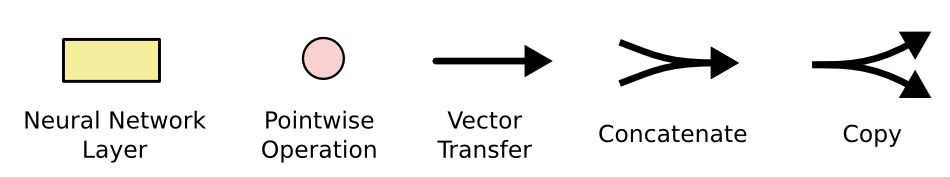
\includegraphics[width=1\textwidth]{nn_lstm_notation}
        \caption{Image notation}
        \label{fig:nn_lstm_notation}
	\end{subfigure}
    \caption{Difference between a standard RNN cell and a LSTM cell (from \textit{colah's blog})}
    \label{fig:rnn_vs_lstm}
\end{figure}

An LSTM cell keeps "in memory" two states, one for the short-term memory and the other for the long-term memory, respectively $\mathbf{h}_t$ and $\mathbf{C}_t$.

\begin{figure}[htbp]
    \centering
    \begin{subfigure}[t]{0.8\textwidth}
		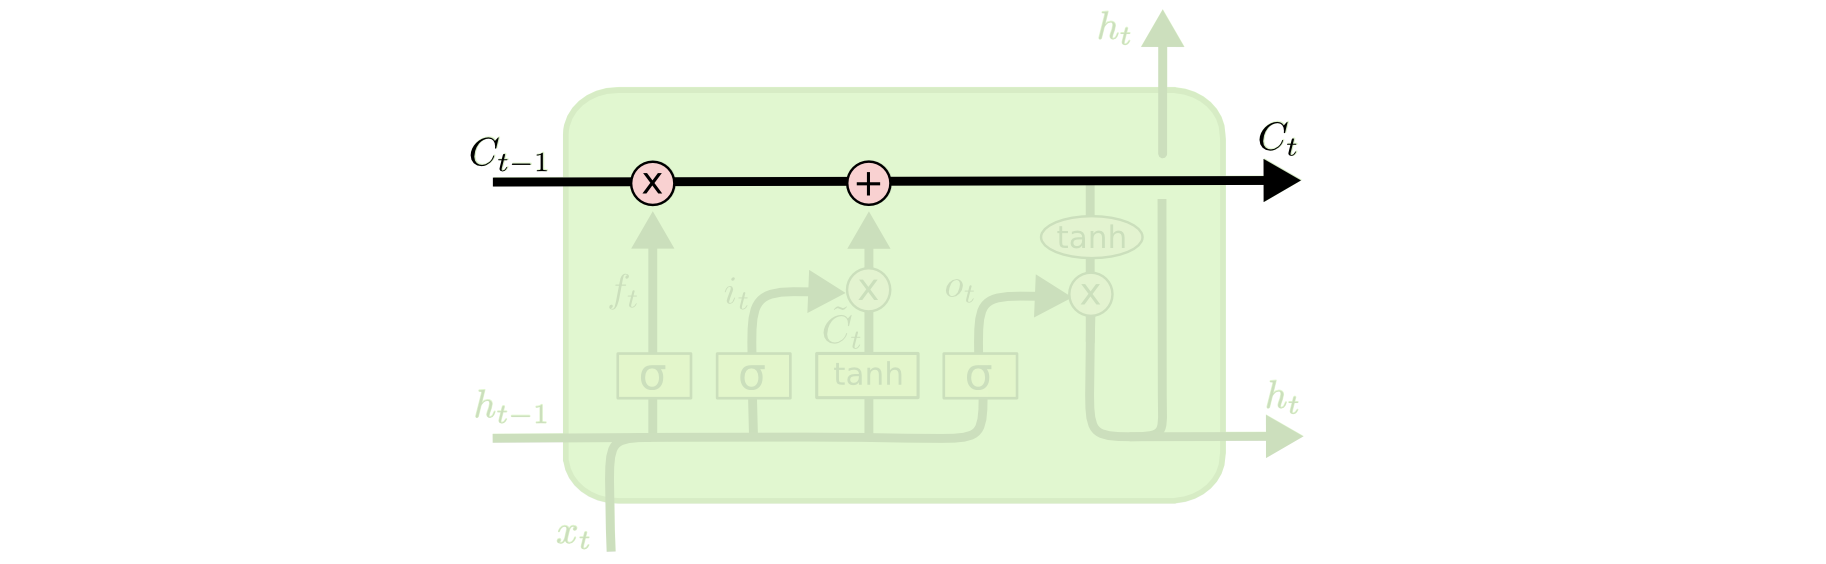
\includegraphics[width=1\textwidth]{nn_lstm_step1}
        \caption{}
        \label{fig:nn_lstm_step1}
	\end{subfigure}
	~
	\begin{subfigure}[t]{0.8\textwidth}
		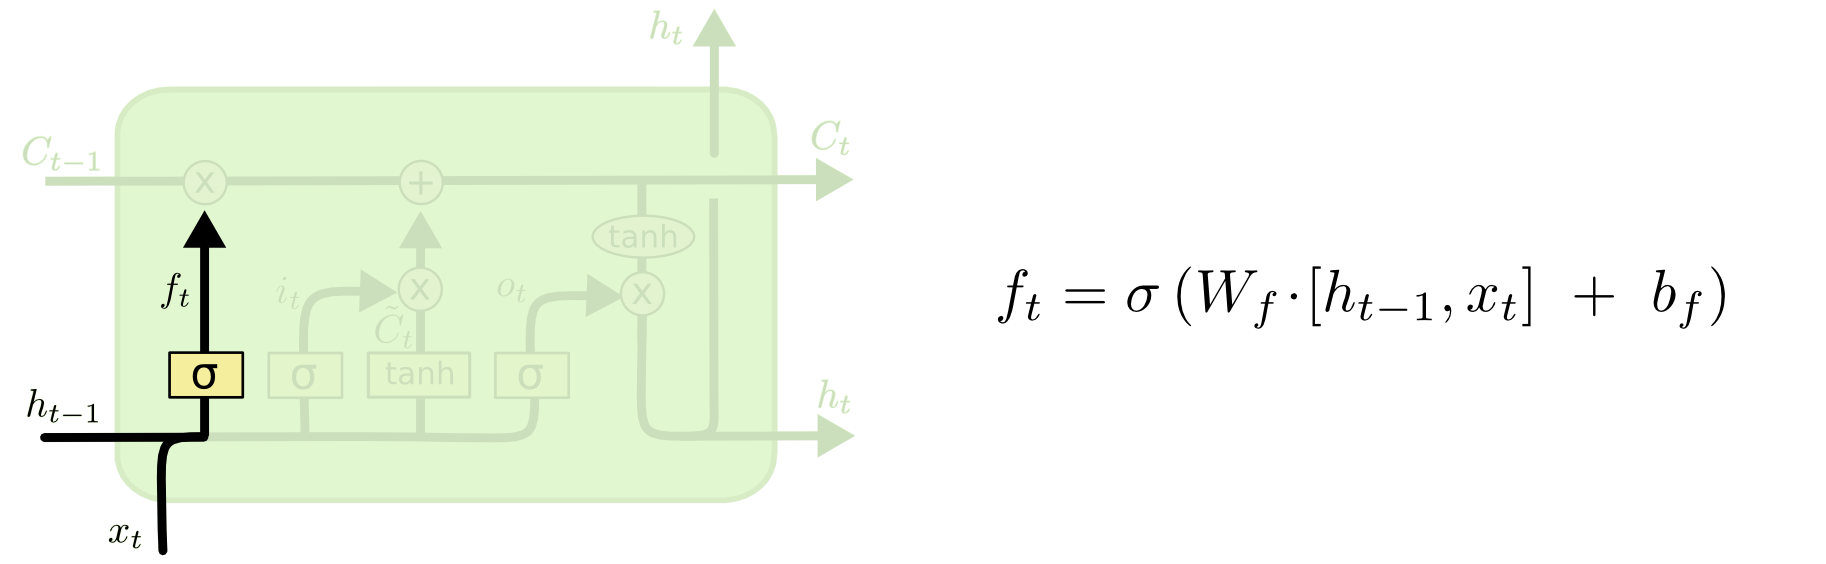
\includegraphics[width=1\textwidth]{nn_lstm_step2}
        \caption{}
        \label{fig:nn_lstm_step2}
    \end{subfigure}
    ~
    \begin{subfigure}[t]{0.8\textwidth}
		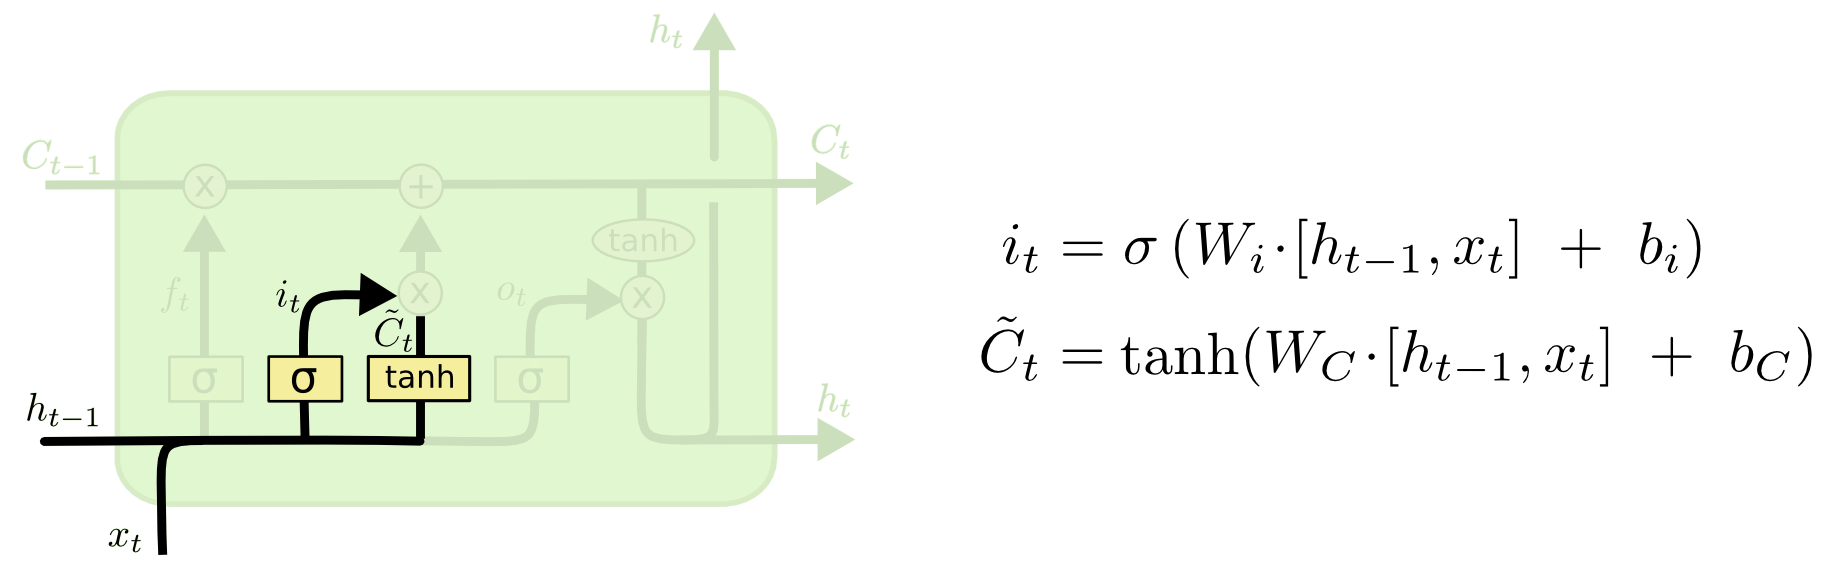
\includegraphics[width=1\textwidth]{nn_lstm_step3}
        \caption{}
        \label{fig:nn_lstm_step3}
    \end{subfigure}
    ~
    \begin{subfigure}[t]{0.8\textwidth}
		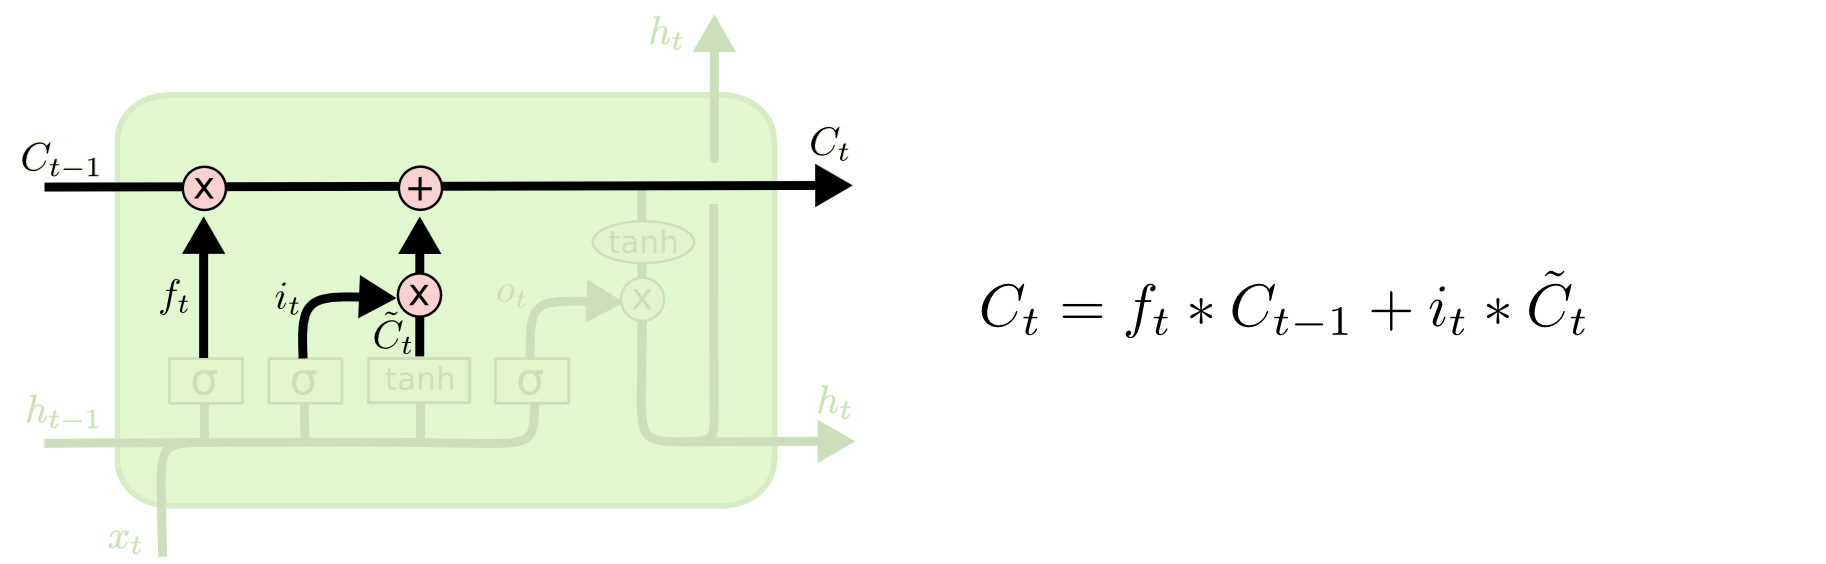
\includegraphics[width=1\textwidth]{nn_lstm_step4}
        \caption{}
        \label{fig:nn_lstm_step4}
    \end{subfigure}
    ~
    \begin{subfigure}[t]{0.8\textwidth}
		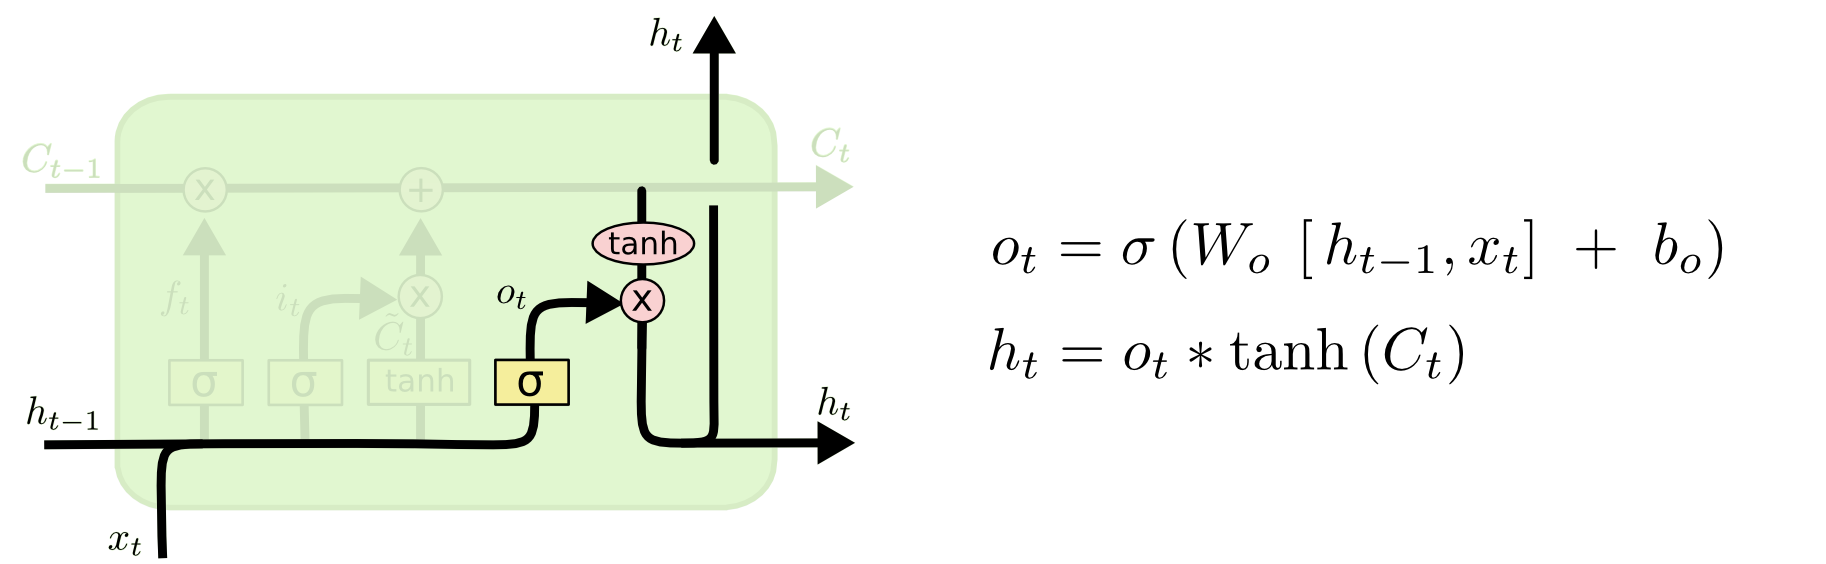
\includegraphics[width=1\textwidth]{nn_lstm_step5}
        \caption{}
        \label{fig:nn_lstm_step5}
    \end{subfigure}
    \caption{Elements in an LSTM cell step-by-step (from \textit{colah's blog})}
    \label{fig:lstm_steps}
\end{figure}

\subsection{Convolutional neural network}

\section{Functional connectivity and graph representation}
\subsection{Functional connectivity}
\subsection{Graph representation}

\section{Graph-based deep learning models}
\subsection{Graph neural network}
\subsection{Edge-conditioned convolution}
\subsection{Global pooling}
\subsection{Graph-based LSTM and Convolutional neural networks}